
\chapter{覆叠}

\section{纤维积与笛卡尔方块}

\subsection{B-空间的结构}

设 B 为一个拓扑空间。

定义 1. --- 拓扑 B-空间（或简称 B-空间）是指一个拓扑空间 X，连同一个从 X 到 B 的连续映射 p。映射 p 称为 B-空间 X 的投影。

设 X、X' 为 B-空间，p、\(p'\) 为它们各自的投影。从 X 到 X' 的 B-态射是指一个从 X 到 X' 的连续映射 f，使得 \(p' \circ f = p\) 。

为方便起见，有时用 \((X,p)\) 表示给拓扑空间 X 装备连续映射 p 之后所得到的 B-空间。

两个 B-态射的复合是一个 B-态射。B-空间的同构也称为 B-同构，它们是作为同胚的那些 B-态射。

这样，如果把集合 X 上的 B-空间结构称为由 X 上的一个拓扑与一个连续映射 \(p: X \rightarrow B\) 所组成的数据，那么就可以取 B-态射作为 B-空间结构的态射 (E, IV, p. 11)。

设 X、\(X'\) 为 B-空间。用 \(\mathcal{C}_{\mathrm{B}}(\mathrm{X};\mathrm{X}')\) 表示从 X 到 \(X'\) 的 B-态射所成的集，用 \(\operatorname{Isom}_{\mathrm{B}}(\mathrm{X};\mathrm{X}')\) 表示从 X 到 \(X'\) 的 B-同构所成的集，用 \(\operatorname{Aut}_{\mathrm{B}}(\mathrm{X})\) 表示 X 的 B-自同构所成的集，也就是从 X 到 X 的 B-同构。

设 X 为一个 B-空间，p 为其投影。若给 B 装备以 \(Id_{B}\) 为投影的 B-空间结构，则集合 \(\mathcal{C}_{\mathrm{B}}(\mathrm{B};\mathrm{X})\) 就是 p 的连续截面 (E, II, p. 18, def. 11) 全体所成的集。

设 X 为一个 B-空间，p 为其投影，b 为 B 的一点。X 的子空间 \(\overline{p}^{1}(b)\) 称为 X 在 b 上的纤维（或 p 在 b 上的纤维），记作 \(X_{b}\) 。为使从 X 到 B-空间 \(X'\) 的连续映射 f 是一个 B-态射，必须且只需 \(f(\mathrm{X}_{b})\) 含于 \(X_{b}'\) ，对一切 \(b \in B\) 。

设 X 为一个 B-空间，p 为其投影。设 f 为从拓扑空间 B' 到 B 中的一个连续映射。连续映射 \(g: B' \to X\) 若满足 \(p \circ g = f\) ，则称为 f 到 X 中的连续提升。换言之，若给 B′ 装备以 f 为投影的 B-空间结构，则 f 到 X 的连续提升就是从 B′ 到 X 的 B-态射。

\subsection{B-空间上的运算}

设 B 为一个拓扑空间。

设 X 为一个 B-空间，p 为其投影。X 的每个拓扑子空间 Y 都赋有以 \(p \mid Y\) 为投影的 B-空间结构。设 A 为 B 的一个子空间；装备上映射 \(p_{\mathrm{A}}: \overline{p}^{1}(\mathrm{A}) \to \mathrm{A}\) （由 p 过渡到子空间所诱导）之后，拓扑空间 \(\overline{p}^{1}(\mathrm{A})\) 是一个 A-空间。它称为 \((\mathrm{X}, p)\) 在 A 上诱导的 A-空间，有时记作 \(X_{A}\) 。

设 \((\mathrm{X}_{i})_{i\in\mathrm{I}}\) 为一族 B-空间，\(p_{i}\) 为 \(X_{i}\) 的投影。和空间 \(X = \coprod_{i\in I} X_{i}\) (TG, I, p. 15) 装备上映射 \(p: X \to B\) ——它由 \(p(i,x) = p_{i}(x)\) 定义（其中 \(i \in I\) ，\(x \in X_{i}\) ）——之后，是一个 B-空间，称为 B-空间族 \((\mathrm{X}_{i})_{i\in\mathrm{I}}\) 的和。典型单射 \(X_{i} \to X\) 都是 B-态射。

设 X 为一个 B-空间，p 为其投影，并设 R 为 X 上的一个等价关系。用 X/R 表示商空间 (TG, I, p. 20, def. 3)。若映射 \(p: X \rightarrow B\) 与关系 R 相容 (E, II, p. 44)，则由 p 过渡到商所诱导的映射 \(p'\colon X/R \to B\) 是连续的 (TG, I, p. 21, prop. 6)；给 X/R 装备投影 \(p'\) 所得的 B-空间称为 X 关于关系 R 的商 B-空间。

\subsection{两个 B-空间的纤维积}

设 B 为一个拓扑空间，X 与 X′ 为 B-空间，p 与 p′ 为它们各自的投影。用 X ×B X′ 表示 X × X′ 中由偶 \((x, x')\) （满足 \(p(x) = p'(x')\) ）组成的拓扑子空间。映射 \(q: X \times_{B} X' \to B\) 由 \(q(x, x') = p(x)\) 定义，它是连续的。

定义 2. --- 拓扑空间 X × \(_{B}\) X' 称为 X 与 X' 在 B 上的纤维积。给 X × \(_{B}\) X' 装备映射 q 所得的 B-空间称为 X 与 X' 的积 B-空间。

\(X \times_{B} X'\) 关于 \(X \times X'\) 到 X 与 X' 上的投影的限制，仍记作 \(pr_{1}\) 与 \(pr_{2}\) ，称为纤维积的第一投影与第二投影。它们是连续的，并且是 B-态射，因为我们有 \(q = p \circ pr_{1} = p' \circ pr_{2}\) 。

注意，\(X \times_{B} X'\) 即使在 X 与 \(X'\) 非空时也可能是空的：事实上，关系 \(X \times_{B} X' = \varnothing\) 等价于 \(p(X)\) 与 \(p'(X')\) 不相交。

设 Y 为一个 B-空间，\(u\colon\mathrm{Y}\to\mathrm{X}, u'\colon\mathrm{Y}\to\mathrm{X}'\) 为 B-态射。存在唯一的 B-态射 \(v\colon\mathrm{Y}\to\mathrm{X}\times_{\mathrm{B}}\mathrm{X}'\) ，使得 \(\mathrm{pr}_{1}\circ v=u\) 且 \(\mathrm{pr}_{2}\circ v=u'\) （两个 B-空间的积 B-空间的泛性质）：它就是映射 \(y\mapsto(u(y),u'(y))\) （从 Y 到 \(\mathrm{X}\times_{\mathrm{B}}\mathrm{X}'\) 中），有时记作 \((u,u')\) 。

设 X、X'、Y、Y' 为 B-空间，\(f: X \to Y\) 、\(f': X' \to Y'\) 为 B-态射。映射 \((x, x') \mapsto (f(x), f'(x'))\) 是从 \(X \times_{B} X'\) 到 \(Y \times_{B} Y'\) 中的一个 B-态射，记作 \(f \times_{B} f'\) ，称为 f 与 \(f'\) 到纤维积的扩张。

例. --- 1) 设 X 与 X' 为 B-空间；则映射 \((x, x') \mapsto (x', x)\) 定义了从 \(X \times_{B} X'\) 到 \(X' \times_{B} X\) 上的一个 B-同构。

\begin{enumerate}
\def\labelenumi{\arabic{enumi})}
\setcounter{enumi}{1}
\item
  设 X、\(X'\) 、\(X''\) 为 B-空间，p、\(p'\) 、\(p''\) 为它们各自的投影。积 B-空间 \((\mathrm{X} \times_{\mathrm{B}} \mathrm{X}') \times_{\mathrm{B}} \mathrm{X}''\) 是拓扑子空间 \(X \times_{B} X' \times_{B} X''\) （含于 \(X \times X' \times X''\) ），由三元组 \((x, x', x'')\) 组成，这些三元组满足 \(p(x) = p'(x') = p''(x''), \text{ 配备投影 } q: X \times_{B} X' \times_{B} X'' \to B\) ，其中投影由 \(q(x, x', x'') = p(x)\) 定义。
\item
  设 X 为一个 B-空间，p 为其投影。X 与 X 在 B 上的纤维积 \(X \times_{B} X\) 称为 X 的纤维方块。它是 \(X \times X\) 中由偶 \((x, x')\) （其中 \(p(x) = p(x')\) ）组成的子空间，赋有以映射 \((x, x') \mapsto p(x)\) 为投影的 B-空间结构。对角线 \(\Delta_{X}\) （\(X \times X\) 的，见 E, II, p. 13）含于 \(X \times_{B} X\) ；它也称为 \(X \times_{B} X\) 的对角线。映射 \(x \mapsto (x, x)\) （从 X 到 \(X \times_{B} X\) 中）是一个 B-态射，称为对角 B-态射，常记作 \(\delta_{X}\) ；它给出从 X 到 \(\Delta_{X}\) 上的一个 B-同构 (TG, I, p. 25, cor. 2)。
\item
  设 \((\mathrm{B}_{i})_{i\in\mathrm{I}}\) 为一族拓扑空间，且对每个 \(i\in I\) ，设 \((\mathrm{X}_{i},p_{i})\) 与 \((\mathrm{Y}_{i},q_{i})\) 为 \(B_{i}\)-空间。令 \(B=\prod_{i\in I}B_{i}\) 、\(X=\prod_{i\in I}X_{i}\) 与 \(Y=\prod_{i\in I}Y_{i}\) 。拓扑空间 X（相应地，Y）装备上连续映射 \(p=\prod_{i}p_{i}\) （相应地，\(q=\prod_{i}q_{i}\) ）后，是一个 B-空间。借助从 \(\prod_{i}(\mathrm{X}_{i}\times\mathrm{Y}_{i})\) 到 \((\prod_{i}\mathrm{X}_{i})\times(\prod_{i}\mathrm{Y}_{i})=\mathrm{X}\times\mathrm{Y}\) 上的拓扑积的结合性同构 (TG, I, p. 25, prop. 2)，子空间 \(\prod_{i}(\mathrm{X}_{i}\times_{\mathrm{B}_{i}}\mathrm{Y}_{i})\) （\(\prod_{i}(\mathrm{X}_{i}\times\mathrm{Y}_{i})\) 的）等同于 \(X\times_{B}Y\) 。
\item
  设 \((\mathrm{X}_{i})_{i\in\mathrm{I}}\) 与 \((\mathrm{Y}_{j})_{j\in\mathrm{J}}\) 为两族 B-空间。设 X 与 Y 为它们的和。对每个 \((i,j)\in\mathrm{I}\times\mathrm{J}\) ，映射 \((x,y)\mapsto((i,x),(j,y))\) 是从 \(X_{i}\times_{B}Y_{j}\) 到子空间 \((\{i\}\times\mathrm{X}_{i})\times_{\mathrm{B}}(\{j\}\times\mathrm{Y}_{j})\) （\(X\times_{B}Y\) 的）上的一个 B-同构。由于这些子空间构成 \(X\times_{B}Y\) 到开子集的一个分拆，映射
\end{enumerate}

\[
h \colon \coprod_ {(i, j) \in \mathrm{I} \times \mathrm{J}} (\mathrm{X} _ {i} \times_ {\mathrm{B}} \mathrm{Y} _ {j}) \to \mathrm{X} \times_ {\mathrm{B}} \mathrm{Y}
\]

由 \(h((i,j),(x,y)) = ((i,x),(j,y))\) 定义，它是一个 B-同构。

\subsection{换基}

设 B、B' 为拓扑空间，\(f\colon\mathrm{B}^{\prime}\to\mathrm{B}\) 为一个连续映射。设 X 为一个 B-空间。映射 \(f\) 给 B' 装备了一个 B-空间结构，由此可以定义纤维积 \(\mathrm{B}^{\prime}\times_{\mathrm{B}}\mathrm{X}\) 。给它装备上映射 \(\mathrm{pr}_{1}\colon\mathrm{B}^{\prime}\times_{\mathrm{B}}\mathrm{X}\to\mathrm{B}^{\prime}\) ，就得到一个 B'-空间，称为 B-空间 X 经换基 \(f\colon\mathrm{B}^{\prime}\to\mathrm{B}\) （或经沿 f 从 B 到 B' 的换基）诱导的 B'-空间。它也称为 X 在 f 下的逆像 B'-空间。它记作 \(f^{*}(\mathrm{X})\) ，当不致对映射 f 引起混淆时，也记作 \(X_{B'}\) 。

当 B' 是 B 的子空间且 \(f: B' \to B\) 是典型单射时，映射 \((b', x) \mapsto x\) （它从 \(B' \times_{B} X\) 到 \(p^{-1}(B')\) 上，其中 p 是 X 的投影）是从 \(f^{*}(X)\) 到 X 在 B' 上诱导的 B'-空间上的一个 B'-同构。

设 Y 为另一个 B-空间，\(u\colon X\to Y\) 为一个 B-态射。映射 \(\mathrm{Id}_{\mathrm{B}^{\prime}}\times_{\mathrm{B}}u\colon \mathrm{B}^{\prime}\times_{\mathrm{B}}\mathrm{X}\to \mathrm{B}^{\prime}\times_{\mathrm{B}}\mathrm{Y}\) 是一个 \(\mathrm{B}'\) -态射，称为 \(\mathrm{B}'\) -态射，也就是由 B-态射 \(u\) 经换基 \(f\colon \mathrm{B}'\to \mathrm{B}\) 诱导而得者，有时记作 \(f^{*}(u)\) ，或记作 \(u_{\mathrm{B}'}\) （当不致对映射 \(f\) 引起混淆时）。它是唯一的 \(\mathrm{B}'\) -态射 \(v\) ，从 \(\mathrm{B}'\times_{\mathrm{B}}\mathrm{X}\) 到 \(\mathrm{B}'\times_{\mathrm{B}}\mathrm{Y}\) 中且满足 \(\mathrm{pr}_2\circ v = u\circ \mathrm{pr}_2\) 。

设 B'' 为一个拓扑空间，\(g: B'' \to B'\) 为一个连续映射。则由 \((b'', (b', x)) \mapsto (b'', x)\) 给出的映射是从 \(g^{*}(f^{*}(\mathrm{X}))\) 到 \((f \circ g)^{*}(\mathrm{X})\) 上的 B''-空间的一个典型同构。

\subsection{一族 B-空间的纤维积}

设 \((\mathrm{X}_{i})_{i\in\mathrm{I}}\) 为一族 B-空间，\(p_{i}\colon X_{i}\to B\) 为它们的投影。用 \(\prod_{B}X_{i}\) 表示 \(B\times\prod_{i\in I}X_{i}\) 中由这样的偶 \((b,(x_{i})_{i\in\mathrm{I}})\) 组成的拓扑子空间：这些偶满足 \(p_{i}(x_{i})=b\) ，对一切 \(i\in I\) 。映射 \(p\colon\prod_{B}X_{i}\to B\) 由 \(p(b,(x_{i})_{i\in\mathrm{I}})=b\) 定义，它是连续的。

定义 3. --- 拓扑空间 \(\prod_{\mathrm{B}} \mathrm{X}_i\) 称为族 \((\mathrm{X}_i)_{i \in \mathrm{I}}\) 在 B 上的纤维积。给 \(\prod_{\mathrm{B}} \mathrm{X}_i\) 装备映射 p 所得的 B-空间称为族 \((\mathrm{X}_i)_{i \in \mathrm{I}}\) 的积 B-空间。

设 \(j \in I\) 。映射 \((b, x) \mapsto \operatorname{pr}_j(x)\) （从 \(\prod_B X_i\) 到 \(X_j\) 中）称为纤维积的指标为 \(j\) 的投影，仍记作 \(\operatorname{pr}_j\) 。它是连续的。它是一个 B-态射，因为有 \(p = p_j \circ \operatorname{pr}_j\) 。

设 Y 为一个 B-空间，q 为其投影。对每个 \(i \in I\) ，设 \(u_i \colon Y \to X_i\) 为一个 B-态射。存在唯一的 B-态射 \(v \colon Y \to \prod_{B} X_i\) ，使得 \(pr_i \circ v = u_i\) 对一切 \(i \in I\) 成立（积 B-空间的泛性质）：它就是从 Y 到 \(\prod_{B} X_i\) 中的映射，由 \(y \mapsto (q(y), (u_i(y))_{i \in I})\) 定义，有时记作 \((u_i)_{i \in I}\) 。

设 \((\mathrm{X}_{i})_{i\in\mathrm{I}}\) 与 \((\mathrm{Y}_{i})_{i\in\mathrm{I}}\) 为两族 B-空间，且对每个 \(i\in I\) ，设 \(f_{i}\colon X_{i}\to Y_{i}\) 为一个 B-态射。映射 \((b,(x_{i})_{i\in\mathrm{I}})\mapsto(b,(f_{i}(x_{i}))_{i\in\mathrm{I}})\) 是从 \(\prod_{B}X_{i}\) 到 \(\prod_{B}Y_{i}\) 中的一个 B-态射，记作 \(\prod_{B}f_{i}\) ，称为族 \((f_{i})_{i\in\mathrm{I}}\) 到纤维积的扩张。

例. --- 1) 当集合 I 为空集时，集合 \(\prod_{i\in I}X_i\) 只有一个元素，而 B-空间 \(\prod_{B}X_{i}\) 等同于 B（装备上投影 \(Id_B\) ）。

\begin{enumerate}
\def\labelenumi{\arabic{enumi})}
\setcounter{enumi}{1}
\item
  当 I 非空时，映射 \((b,x)\mapsto x\) （从 \(B\times\prod_{i\in I}X_{i}\) 到 \(\prod_{i\in I}X_{i}\) 中）通过过渡到子空间诱导出一个同胚，从 \(\prod_{B}X_{i}\) 到 \(\prod_{i\in I}X_{i}\) 的由族 \((x_{i})_{i\in I}\) 组成的子空间上，这些族满足 \(p_{i}(x_{i})=p_{j}(x_{j})\) ，对一切 \(i,j\in I\) 。今后称这个子空间为族 \((\mathrm{X}_{i})_{i\in\mathrm{I}}\) 的纤维积（滥用用语）。
\item
  当集合 I 只有一个元素 \(\alpha\) （相应地，两个元素 \(\alpha\) 与 \(\beta\) ；相应地，三个元素 \(\alpha\) 、\(\beta\) 、\(\gamma\) ）时，映射 \(\mathrm{pr}_{\alpha}\) （相应地，\((\mathrm{pr}_{\alpha}, \mathrm{pr}_{\beta})\) ；相应地，\((\mathrm{pr}_{\alpha}, \mathrm{pr}_{\beta}, \mathrm{pr}_{\gamma})\) ）——从 \(\prod_{\mathrm{B}} \mathrm{X}_i\) 到 \(\mathrm{X}_{\alpha}\) （相应地，到 \(\mathrm{X}_{\alpha} \times_{\mathrm{B}} \mathrm{X}_{\beta}\) ；相应地，到 \(\mathrm{X}_{\alpha} \times_{\mathrm{B}} \mathrm{X}_{\beta} \times_{\mathrm{B}} \mathrm{X}_{\gamma}\) ）中——是一个 B-同构。这将使我们能够从 B-空间族的纤维积的性质推出两个或三个 B-空间的纤维积的性质。
\end{enumerate}

设 \((\mathrm{X}_{i})_{i\in\mathrm{I}}\) 为一族 B-空间，J 为 I 的一个子集。由映射 \(Id_{B}\times pr_{J}\) （从 \(B\times\prod_{i\in I}X_{i}\) 到 \(B\times\prod_{i\in J}X_{i}\) 中）通过过渡到子集，得到一个 B-态射 \(\prod_{i\in I}X_{i}\to\prod_{i\in J}X_{i}\) 。我们仍把它记作 \(pr_{J}\) ，称之为纤维积的指标为 J 的投影。

设 \((\mathrm{X}_{i})_{i\in\mathrm{I}}\) 为一族 B-空间。设 \((\mathrm{J}_{\lambda})_{\lambda\in\mathrm{L}}\) 为 I 的一个分拆。映射 \((\mathrm{pr}_{\mathrm{J}_{\lambda}})_{\lambda\in\mathrm{L}}\) （从 \(\prod_{i\in I}X_{i}\to\prod_{\lambda\in L}\left(\prod_{i\in J_{\lambda}}X_{i}\right)\) ）是一个 B-同构（B-空间的纤维积的“结合性”）。

\subsection{笛卡尔方块}

设 B、B′、X、X′ 为拓扑空间，\(f: B' \to B\) 、\(f': X' \to X\) 、\(p: X \to B\) 、\(p': X' \to B'\) 为连续映射。这样的四元组 \((f, f', p, p')\) 可以用一个图示来表示

\begin{enumerate}
\def\labelenumi{(\arabic{enumi})}
\tightlist
\item
\end{enumerate}

\pandocbounded{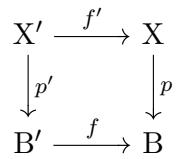
\includegraphics[keepaspectratio]{images/part001_dd3067cf.jpg}}

(E, II, p. 14). 于是我们说“考虑方块图 (1)”，或简单地说“方块 (1)”，以代替说“考虑连续映射的四元组 \(f,f^{\prime},p,p^{\prime}\) ”。称方块 (1) 为交换的，如果等式

\[
f \circ p ^ {\prime} = p \circ f ^ {\prime}
\]

成立。在这情形下，常给 B′、X 与 X′ 分别装备由映射 f、p 与 \(f \circ p' = p \circ f'\) 所定义的 B-空间结构；此时映射 \(p'\) 与 \(f'\) 是 B-态射。

定义 4. --- 我们称方块 (1) 为拓扑空间的笛卡尔方块（或简单地称它是笛卡尔的），如果它是交换的，并且对每个拓扑空间 Y 和每对连续映射 u: Y → B' 与 v: Y → X（满足 f ∘ u = p ∘ v），存在唯一的连续映射 w: Y → X'，满足 p' ∘ w = u 且 f' ∘ w = v。

为使方块 (1) 是笛卡尔的，必须且只需方块

(1')

\pandocbounded{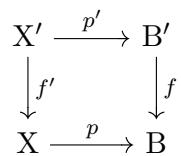
\includegraphics[keepaspectratio]{images/part001_f0fdde30.jpg}}

是笛卡尔的。

命题 1. --- 为使方块 (1) 是笛卡尔的，必须且只需它是交换的，并且对每个 B-空间 Y 和每对 B-态射 \(u\colon Y \to B'\) 、\(v\colon Y \to X\) ，存在唯一的 B-态射 \(w\colon Y \to X'\) ，使得 \(p' \circ w = u\) 且 \(f' \circ w = v\) 。

设方块 (1) 是笛卡尔的。设 Y 为一个 B-空间，\(u: Y \to B'\) 与 \(v: Y \to X\) 为 B-态射。映射 \(f \circ u\) 与 \(p \circ v\) 都等于 B-空间 Y 的投影；于是满足 \(p' \circ w = u\) 与 \(f' \circ w = v\) 的唯一连续映射 w 是一个 B-态射。这就证明了条件的必要性。

反之，设此条件成立。设 Y 为一个拓扑空间，\(u \colon \mathrm{Y} \to \mathrm{B}'\) 与 \(v \colon \mathrm{Y} \to \mathrm{X}\) 为满足 \(f \circ u = p \circ v\) 的连续映射。当 Y 装备上由 \(f \circ u\) 定义的 B-空间结构时，\(u\) 与 \(v\) 是 B-态射。每个连续映射 \(w \colon \mathrm{Y} \to \mathrm{X}'\) ，只要满足 \(p' \circ w = u\) 与 \(f' \circ w = v\) ，就是一个 B-态射，所以这样的映射恰好存在一个。

命题 2. --- 设 B、B' 与 X 为拓扑空间，p: X → B、f: B' → B 为连续映射。

\begin{enumerate}
\def\labelenumi{\alph{enumi})}
\tightlist
\item
  方块
\end{enumerate}

\[
\begin{array}{c} \mathrm{B} ^ {\prime} \times_ {\mathrm{B}} \mathrm{X} \xrightarrow {\mathrm{pr} _ {2}} \mathrm{X} \\ \Biggl \downarrow \mathrm{pr} _ {1} \\ \mathrm{B} ^ {\prime} \xrightarrow {f} \mathrm{B} \end{array}\tag{2}
\]

是一个笛卡尔方块。

\begin{enumerate}
\def\labelenumi{\alph{enumi})}
\setcounter{enumi}{1}
\tightlist
\item
  对每个交换方块
\end{enumerate}

\[
\begin{array}{c} \mathrm {X^ {\prime}} \xrightarrow {f ^ {\prime}} \mathrm{X} \\ \Big \downarrow_ {p ^ {\prime}} \\ \mathrm {B^ {\prime}} \xrightarrow {f} \mathrm{B} \end{array}\tag{3}
\]

存在唯一的连续映射 \(h: X' \to B' \times_{B} X\) ，使得 \(pr_{1} \circ h = p'\) 且 \(pr_{2} \circ h = f'\) 。

\begin{enumerate}
\def\labelenumi{\alph{enumi})}
\setcounter{enumi}{2}
\tightlist
\item
  交换方块 (3) 是笛卡尔的，当且仅当 h 是一个同胚。
\end{enumerate}

断言 \(a\) ) 由命题 1 以及 B-空间的范畴中两个 B-空间的积的泛性质 (I, p. 3) 得出。断言 \(b\) ) 由它得出。

若方块 (3) 是笛卡尔的，则存在唯一的连续映射 \(h'\colon B'\times_{B}X\to X'\) ，使得 \(f'\circ h' = pr_{2}\) 且 \(p'\circ h' = pr_{1}\) 。我们有 \(f'\circ h'\circ h = f'\) 与 \(p'\circ h'\circ h = p'\) ，由于方块 (3) 是笛卡尔的，从而 \(h'\circ h = Id_{X'}\) 。我们有 \(pr_{1}\circ h\circ h' = pr_{1}\) 与 \(pr_{2}\circ h\circ h' = pr_{2}\) ，由于方块 (2) 是笛卡尔的，从而 \(h\circ h' = Id_{B'\times_{B}X}\) 。这就证明了 h 是一个同胚。

反之，设 h 是一个同胚；由于方块 (2) 是笛卡尔的，方块 (3) 也是笛卡尔的。

映射 \(h \colon \mathrm{X}' \to \mathrm{B}' \times_{\mathrm{B}} \mathrm{X}\) ——其存在性与唯一性由前一命题的 \(b)\) 款所断言——将称为典型的：它就是在 I, p. 3 中记作 \((p', f')\) 的映射。

命题 3. --- 设

\[
\begin{array}{c} \mathrm {X^ {\prime}} \xrightarrow {f ^ {\prime}} \mathrm{X} \\ \Big \downarrow_ {p ^ {\prime}} \\ \mathrm {B^ {\prime}} \xrightarrow {f} \mathrm{B} \end{array}
\]

为一个笛卡尔方块。对 \(p'\) 的任一连续截面 s，映射 \(f'\circ s\) 是 f 到 X 中的连续提升。映射 \(s\mapsto f'\circ s\) 是从 \(\mathcal{C}_{\mathrm{B}'}(\mathrm{B}';\mathrm{X}')\) 到 \(\mathcal{C}_{\mathrm{B}}(\mathrm{B}';\mathrm{X})\) 上的一个双射。

若 \(s \colon B' \to X'\) 是 \(p'\) 的一个连续截面，我们有 \(p \circ f' \circ s = f \circ p' \circ s = f\) ，这就证明 \(f' \circ s\) 是 \(f\) 到 X 中的连续提升，即从 \(B'\) 到 X 中的一个 B-态射。反之，设 \(g \colon B' \to X\) 是一个 B-态射。我们有 \(f \circ \mathrm{Id}_{\mathrm{B}'} = p \circ g\) ；于是由笛卡尔方块的定义，存在唯一的连续映射 \(s \colon B' \to X'\) ，使得 \(p' \circ s = \mathrm{Id}_{\mathrm{B}'}\) 且 \(f' \circ s = g\) ，命题得证。

\subsection{由过渡到子空间构造的笛卡尔方块}

命题 4. --- 设

\[
\begin{array}{c} \mathrm {X^ {\prime}} \xrightarrow {f ^ {\prime}} \mathrm{X} \\ \Big \downarrow_ {p ^ {\prime}} \\ \mathrm {B^ {\prime}} \xrightarrow {f} \mathrm{B} \end{array}\tag{4}
\]

为一个笛卡尔方块，并设 \(B_{0}\) 、\(B_{0}^{\prime}\) 、\(X_{0}\) 分别为 B、\(B^{\prime}\) 与 X 的子空间。设 \(f(B_{0}^{\prime}) \subset B_{0}\) ，\(p(X_{0}) \subset B_{0}\) ，并令 \(X_{0}^{\prime} = \overline{p'}^{1}(B_{0}^{\prime}) \cap \overline{f'}^{1}(X_{0})\) 。则方块

\[
\begin{array}{c} \mathrm{X} _ {0} ^ {\prime} \xrightarrow {f _ {0} ^ {\prime}} \mathrm{X} _ {0} \\ \Biggl \downarrow p _ {0} ^ {\prime} \\ \mathrm{B} _ {0} ^ {\prime} \xrightarrow {f _ {0}} \mathrm{B} _ {0} \end{array}\tag{4'}
\]

（其中映射 \(f_0\) 、\(f_0'\) 、\(p_0\) 、\(p_0'\) 分别由 \(f\) 、\(f'\) 、\(p\) 、\(p'\) 过渡到子集得到）是笛卡尔的。

考虑由交换图 (4) 得到的典型映射 \(h \colon X' \to B' \times_B X\) 。由于方块 (4) 是笛卡尔的，\(h\) 是一个同胚。按构造，我们有 \(X_0' = h^{-1}(B_0' \times_{B_0} X_0)\) ，而映射 \(h_0 \colon X_0' \to B_0' \times_{B_0} X_0\) 由交换图 ( \(4'\) ) 得到，它是由 \(h\) 过渡到子集得到的。因此它是一个同胚，从而方块 ( \(4'\) ) 是笛卡尔的 (prop. 2)。

推论. --- 设

\pandocbounded{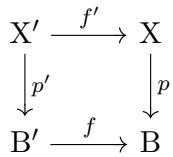
\includegraphics[keepaspectratio]{images/part001_2907af81.jpg}}

为一个笛卡尔方块。

\begin{enumerate}
\def\labelenumi{\alph{enumi})}
\item
  对每个点 \(b'\) （在 \(B'\) 中），映射 \(f'\) 诱导出纤维 \(X_{b'}'\) （\(p'\) 的）到纤维 \(X_{f(b')}\) （\(p\) 的）上的一个同胚。
\item
  若映射 p 是单射（相应地，满射；相应地，双射），则 \(p'\) 亦然。
\end{enumerate}

设 \(b'\) 为 B' 的一点。令 \(b = f(b')\) 。对一切 \(x' \in X_{b'}'\) ，我们有 \(p(f'(x')) = f(p'(x')) = f(b') = b\) ，从而 \(f'(x') \in X_b\) 。这就证明 \(X_{b'}' \subset \overline{f'}^{1}(X_b)\) 。在命题 4 中取 \(B_0 = \{b\}\) 、\(B_0' = \{b'\}\) 与 \(X_0 = X_b\) ；于是有 \(X_0' = X_{b'}'\) ，由此得断言 \(a\) )。

为使映射 p 是单射（相应地，满射；相应地，双射），必须且只需它的每个纤维的基数至多（相应地，至少；相应地，恰好）是 1。断言 b) 由此得出。

例. --- 设 \((X,p)\) 为一个 B-空间，A 为 B 的一个子空间。方块

\[
\begin{array}{c} \overline {{p}} ^ {1} (\mathrm{A}) \xrightarrow {j} \mathrm{X} \\ \Biggl \downarrow p _ {\mathrm{A}} \\ \mathrm{A} \xrightarrow {i} \mathrm{B} \end{array}\tag{5}
\]

（其中 i 与 j 是典型单射）是笛卡尔的。

特别地，若 A 与 A' 是拓扑空间 B 的子空间，则方块

\begin{enumerate}
\def\labelenumi{(\arabic{enumi})}
\setcounter{enumi}{5}
\tightlist
\item
\end{enumerate}

\pandocbounded{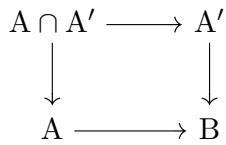
\includegraphics[keepaspectratio]{images/part001_a4278a10.jpg}}

（其中的箭头是典型单射）是笛卡尔的。

\subsection{由积、纤维积与和构造的笛卡尔方块}

命题 5. --- 设 I 为一个集合，且对每个 \(i \in I\) ，设

\[
\begin{array}{c} \mathrm{X} _ {i} ^ {\prime} \xrightarrow {f _ {i} ^ {\prime}} \mathrm{X} _ {i} \\ \Big \downarrow p _ {i} ^ {\prime} \\ \mathrm{B} _ {i} ^ {\prime} \xrightarrow {f _ {i}} \mathrm{B} _ {i} \end{array}\tag{7}
\]

为一个笛卡尔方块。方块

\[
\begin{array}{c} \prod_ {i \in \mathrm{I}} \mathrm{X} _ {i} ^ {\prime} \xrightarrow {f ^ {\prime}} \prod_ {i \in \mathrm{I}} \mathrm{X} _ {i} \\ \Biggl \downarrow^ {p ^ {\prime}} \qquad \qquad \qquad \qquad \Biggl \downarrow^ {p} \\ \prod_ {i \in \mathrm{I}} \mathrm{B} _ {i} ^ {\prime} \xrightarrow {f} \prod_ {i \in \mathrm{I}} \mathrm{B} _ {i} \end{array}\tag{ (7') }
\]

\((\text{其中 } f, f', p, p' \text{ 是这些族 } (f_i), (f'_i), (p_i), (p'_i) \text{ 在乘积上的延拓}) \text{ 是笛卡尔的。}\)

设 Y 为一个拓扑空间，\(u \colon \mathrm{Y} \to \prod_{i} \mathrm{B}_{i}'\) 与 \(v \colon \mathrm{Y} \to \prod_{i} \mathrm{X}_{i}\) 为满足 \(f \circ u = p \circ v\) 的连续映射。对 \(i \in \mathrm{I}\) ，令 \(u_{i} = \mathrm{pr}_{i} \circ u\) 与 \(v_{i} = \mathrm{pr}_{i} \circ v\) ；我们有 \(f_{i} \circ u_{i} = p_{i} \circ v_{i}\) ，且存在唯一的连续映射 \(w_{i} \colon \mathrm{Y} \to \mathrm{X}_{i}'\) ，使得 \(p_{i}' \circ w_{i} = u_{i}\) 且 \(f_{i}' \circ w_{i} = v_{i}\) 。于是映射 \(w = (w_{i})\) 是从 Y 到 \(\prod_{i} \mathrm{X}_{i}'\) 中的一个连续映射，满足 \(p' \circ w = u\) 与 \(f' \circ w = v\) ，并且它是具有这些性质的唯一映射。

推论 1. --- 设 X 为一个 B-空间，p 为其投影，F 为一个拓扑空间。方块

\[
\begin{array}{c} \mathrm{X} \times \mathrm{F} \xrightarrow {\operatorname{pr} _ {1}} \mathrm{X} \\ \Biggl \downarrow p \times \mathrm{Id} _ {\mathrm{F}} \\ \mathrm{B} \times \mathrm{F} \xrightarrow {\operatorname{pr} _ {1}} \mathrm{B} \end{array}\tag{8}
\]

是笛卡尔的。

设 P 为化约为一点的空间。推论 1 由把命题 5 应用于下列笛卡尔方块而得

\[
\begin{array}{l} \mathrm{X} \xrightarrow {\mathrm{Id} _ {\mathrm{X}}} \mathrm{X} \\ \Big \downarrow_ {p} \qquad \Big \downarrow_ {p} \\ \mathrm{B} \xrightarrow {\mathrm{Id} _ {\mathrm{B}}} \mathrm{B} \end{array} \qquad \text {and} \qquad \begin{array}{l} \mathrm{F} \longrightarrow \mathrm{P} \\ \Big \downarrow_ {\mathrm{Id} _ {\mathrm{F}}} \qquad \Big \downarrow_ {\mathrm{Id} _ {\mathrm{P}}} \\ \mathrm{F} \longrightarrow \mathrm{P}. \end{array}
\]

设 B 与 B' 为拓扑空间，\(f: B' \to B\) 为一个连续映射。设 I 为一个集合，且对每个 \(i \in I\) ，设 \(X_i\) 为一个 B-空间，\(X'_i\) 为一个 B'-空间，\(f'_i: X'_i \to X_i\) 为一个连续映射，使得方块

\[
\begin{array}{c} \mathrm{X} _ {i} ^ {\prime} \xrightarrow {f _ {i} ^ {\prime}} \mathrm{X} _ {i} \\ \Big \downarrow \\ \mathrm{B} ^ {\prime} \xrightarrow {f} \mathrm{B} \end{array}\tag{9}
\]

是交换的。存在唯一的连续映射

\[
f ^ {\prime} \colon \prod_ {i \in \mathrm{I}} \mathrm{X} _ {i} ^ {\prime} \to \prod_ {i \in \mathrm{I}} \mathrm{X} _ {i}
\]

满足 \(pr_{i} \circ f' = f_{i}' \circ pr_{i}\) （对一切 \(i \in I\) ），且使得方块

\[
\begin{array}{c} \prod_ {i \in I} X _ {i} ^ {\prime} \xrightarrow {f ^ {\prime}} \prod_ {i \in I} X _ {i} \\ \Big \downarrow \qquad \qquad \qquad \qquad \Big \downarrow \\ B ^ {\prime} \xrightarrow {f} B \end{array}\tag{ (9') }
\]

是交换的（若 I ≠ ∅，这最后一个条件可由其余条件推出）：它是由映射

\[
f \times \prod_ {i \in \mathrm{I}} f _ {i} ^ {\prime} \colon \mathrm{B} ^ {\prime} \times \prod_ {i \in \mathrm{I}} \mathrm{X} _ {i} ^ {\prime} \to \mathrm{B} \times \prod_ {i \in \mathrm{I}} \mathrm{X} _ {i}
\]

过渡到子集而得到的。在这些记号下：

推论 2. --- 若对每个 \(i \in I\) 方块 (9) 都是笛卡尔的，则方块 ( \(9'\) ) 是笛卡尔的。

由命题 5 推出一个笛卡尔方块

\[
\begin{array}{c} \mathrm{B} ^ {\prime} \times \prod_ {i} \mathrm{X} _ {i} ^ {\prime} \xrightarrow {\operatorname{Id} _ {\mathrm{B}} \times \prod_ {i} f _ {i} ^ {\prime}} \mathrm{B} \times \prod_ {i} \mathrm{X} _ {i} \\ \Biggl \downarrow \\ \mathrm{B} ^ {\prime} \times (\mathrm{B} ^ {\prime}) ^ {\mathrm{I}} \xrightarrow {f \times \prod_ {i} f} \mathrm{B} \times \mathrm{B} ^ {\mathrm{I}}  . \end{array}
\]

用 \(\Delta_{\mathrm{B}^{\prime}}\) 与 \(\Delta_{\mathrm{B}}\) 表示 \(\mathrm{B}^{\prime}\times (\mathrm{B}^{\prime})^{\mathrm{I}}\) 与 \(\mathrm{B}\times \mathrm{B}^{\mathrm{I}}\) 的对角线。图表

\[
\begin{array}{c} \prod_ {i \in \mathrm{I}} X _ {i} ^ {\prime} \xrightarrow {f ^ {\prime}} \prod_ {i \in \mathrm{I}} X _ {i} \\ \Big \downarrow \qquad \qquad \qquad \Big \downarrow \\ \Delta_ {\mathrm{B} ^ {\prime}} \xrightarrow {} \Delta_ {\mathrm{B}} \end{array}
\]

由前一个图表过渡到子空间得到，它是笛卡尔的 (I, p. 9, prop. 4)。它等同于图表 (9')。

例 1. --- 设

\[
\begin{array}{c} \mathrm {X^ {\prime}} \xrightarrow {f ^ {\prime}} \mathrm{X} \\ \Big \downarrow_ {p ^ {\prime}} \\ \mathrm {B^ {\prime}} \xrightarrow {f} \mathrm{B} \end{array}
\]

为一个笛卡尔方块。于是推论 2 给出一个笛卡尔方块

\[
\begin{array}{c} \mathrm {X^ {\prime} \times_ {B^ {\prime}} X^ {\prime}} \xrightarrow {\varphi} \mathrm {X\times_ {B} X} \\ \Big \downarrow \\ \mathrm {B^ {\prime} \xrightarrow {f} B}. \end{array}
\]

我们有关系式 \(\overline{\varphi}^{1}(\Delta_{\mathrm{X}}) = \Delta_{\mathrm{X}^{\prime}}\) 。事实上，由 I, p. 8 的命题 2，只需考虑 \(\mathrm{X}' = \mathrm{B}' \times_{\mathrm{B}} \mathrm{X}\) 的情形。设 \(((b,x),(b,x'))\) 为 \(X^{\prime} \times_{B^{\prime}} X^{\prime}\) 的一个元素，其中 \(b \in B^{\prime}\) ，\(x, x^{\prime} \in X\) 。这个元素属于 \(\overline{\varphi}^{1}(\Delta_{\mathrm{X}})\) 当且仅当 \(x = x^{\prime}\) 。

命题 6. --- 设 I 为一个集合，且对每个 \(i \in I\) ，设

\[
\begin{array}{c} \mathrm{X} _ {i} ^ {\prime} \xrightarrow {f _ {i} ^ {\prime}} \mathrm{X} \\ \Biggl \downarrow p _ {i} ^ {\prime} \\ \mathrm{B} _ {i} ^ {\prime} \xrightarrow {f _ {i}} \mathrm{B} \end{array}\tag{10}
\]

为一个笛卡尔方块。设 X' 与 B' 分别为族 \((X'_i)\) 与 \((B'_i)\) 的和空间。设 f: B' → B、f': X' → X 与 p': X' → B' 为分别由族 \((f_i)\) 、\((f'_i)\) 与 \((p'_i)\) 诱导出的映射。方块

\((10')\)

\pandocbounded{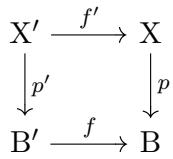
\includegraphics[keepaspectratio]{images/part001_48571453.jpg}}

是笛卡尔的。

映射 \(f\) 、\(f'\) 与 \(p'\) 都是连续的。方块 \((10')\) 的交换性由其定义得出。设 \(h_i\) 表示从 \(\mathrm{X}_i'\) 到 \(\mathrm{B}_i' \times_{\mathrm{B}} \mathrm{X}\) 上的典型同胚 (I, p. 8, 命题 2)，并设 \(h: \mathrm{X}' \to \mathrm{B}' \times_{\mathrm{B}} \mathrm{X}\) 为典型映射 (loc. cit.)。我们有 \(h = h'' \circ h'\) ，其中 \(h': \mathrm{X}' \to \coprod (\mathrm{B}_i' \times_{\mathrm{B}} \mathrm{X})\) 是由诸 \(h_i\) 诱导的同胚，而 \(h'': \coprod (\mathrm{B}_i' \times_{\mathrm{B}} \mathrm{X}) \to (\coprod \mathrm{B}_i') \times_{\mathrm{B}} \mathrm{X}\) 是在 I, p. 4 的例 5 中定义的那个映射。由 I, p. 8 的命题 2 即得结论。

例 2. --- 设 \((X,p)\) 为一个 B-空间，\((\mathrm{A}_{k})_{k\in\mathrm{K}}\) 为 B 的一族子空间。设 A 为族 \((\mathrm{A}_{k})_{k\in\mathrm{K}}\) 的和空间，Y 为族 \((\overline{p}^{1}(\mathrm{A}_{k}))_{k\in\mathrm{K}}\) 的和空间；用 \(i: A \to B\) 、\(j: Y \to X\) 与 \(p': Y \to A\) 分别表示由 \(A_{k}\) 到 B 中的典型单射、\(\overline{p}^{1}(\mathrm{A}_{k})\) 到 X 中的典型单射以及诸映射 \(p_{\mathrm{A}_{k}}: \overline{p}^{1}(\mathrm{A}_{k}) \to \mathrm{A}_{k}\) （\(k \in K\) ）所诱导的映射。方块

\[
\begin{array}{c} \mathrm{Y} \xrightarrow {j} \mathrm{X} \\ \Biggl \downarrow p ^ {\prime} \\ \mathrm{A} \xrightarrow {i} \mathrm{B} \end{array}\tag{11}
\]

是笛卡尔的；这由 I, p. 10 的例与命题 6 得出。

\subsection{笛卡尔方块的复合}

命题 7. --- 设

\[
\begin{array}{c} \mathrm {X^ {\prime\prime}} \xrightarrow {g ^ {\prime}} \mathrm {X^ {\prime}} \\ \Big \downarrow_ {p ^ {\prime \prime}} \\ \mathrm {B^ {\prime\prime}} \xrightarrow {g} \mathrm {B^ {\prime}} \end{array}\tag{12}
\]

和

\begin{enumerate}
\def\labelenumi{(\arabic{enumi})}
\setcounter{enumi}{12}
\tightlist
\item
\end{enumerate}

\pandocbounded{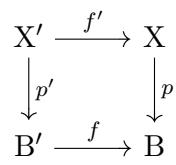
\includegraphics[keepaspectratio]{images/part001_4552bd62.jpg}}

为两个交换方块；考虑方块

\begin{enumerate}
\def\labelenumi{(\arabic{enumi})}
\setcounter{enumi}{13}
\tightlist
\item
\end{enumerate}

\pandocbounded{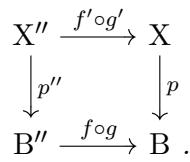
\includegraphics[keepaspectratio]{images/part001_1603e4c4.jpg}}

它是交换的。若方块 (12) 与 (13) 都是笛卡尔的，则方块 (14) 亦然。若方块 (13) 与 (14) 都是笛卡尔的，则方块 (12) 亦然。

方块 (14) 是交换的，因为我们有 \(p \circ f' \circ g' = f \circ p' \circ g' = f \circ g \circ p''\) 。用 \(h' : X'' \to B'' \times_{B'} X'\) 、\(h : X' \to B' \times_{B} X\) 与 \(h'' : X'' \to B'' \times_{B} X\) 表示分别由交换方块 (12)、(13) 与 (14) 得到的典型连续映射。此外，用

\[
j \colon \mathrm{B} ^ {\prime \prime} \times_ {\mathrm{B}} \mathrm{X} \rightarrow \mathrm{B} ^ {\prime \prime} \times_ {\mathrm{B} ^ {\prime}} (\mathrm{B} ^ {\prime} \times_ {\mathrm{B}} \mathrm{X})
\]

表示把 \((b'', x)\) 映为 \((b'', g(b''), x)\) 的连续映射。它是一个同胚，并且有 \(j \circ h'' = (\mathrm{Id}_{\mathrm{B}''} \times_{\mathrm{B}} h) \circ h'\) 。

设方块 (13) 是笛卡尔的。于是 h 是一个同胚 (I, p. 8, prop 2)，从而映射 \(Id_{B''} \times_{B} h\) 是一个同胚，并且 \(h''\) 是同胚当且仅当 \(h'\) 是同胚。这就是说，方块 (12) 是笛卡尔的当且仅当方块 (14) 是笛卡尔的 (loc. cit.)。

采用命题 7 中的记号，有时称方块 (14) 为方块 (13) 与 (12) 的复合方块。第一个断言表明：两个笛卡尔方块的复合是笛卡尔的。特别地，B''-空间 \(g^{*}(f^{*}(\mathrm{X}))\) 与 \((f \circ g)^{*}(\mathrm{X})\) 是同构的。

\pandocbounded{
\includegraphics[keepaspectratio]{images/part001_52f28a70.jpg}}

注. --- 1) 可能发生这样的情形：方块 (12) 与 (14) 都是笛卡尔的，而方块 (13) 却不是 (I, p. 139, exerc. 2)。

\begin{enumerate}
\def\labelenumi{\arabic{enumi})}
\setcounter{enumi}{1}
\tightlist
\item
  设 \(p \colon \mathrm{X} \to \mathrm{B}\) 与 \(f \colon \mathrm{B}' \to \mathrm{B}\) 为连续映射。映射 \(g \colon \mathrm{B}' \to \mathrm{B}' \times \mathrm{B}\) （由 \(g(b') = (b', f(b'))\) 定义）是从 \(\mathrm{B}'\) 到图像 \(\mathrm{G}\) （映射 \(f\) 的）上的一个同胚 (TG, I, p. 25, cor. 2)，而纤维积 \(\mathrm{B}' \times_{\mathrm{B}} \mathrm{X}\) 可以等同 (I, p. 6) 于 \(\mathrm{B}' \times \mathrm{X}\) 的一个子空间，即 \(\mathrm{G}\) 在映射 \(\mathrm{Id}_{\mathrm{B}'} \times p \colon \mathrm{B}' \times \mathrm{X} \to \mathrm{B}' \times \mathrm{B}\) 下的原像。由 I, p. 10 的例与命题 5 的推论 1 (I, p. 11)，方块
\end{enumerate}

\[
\begin{array}{c c} \mathrm {B^ {\prime}} \times_ {\mathrm{B}} \mathrm{X} \xrightarrow {i} \mathrm {B^ {\prime}} \times \mathrm{X} & \mathrm {B^ {\prime}} \times \mathrm{X} \xrightarrow {\mathrm{pr} _ {2}} \mathrm{X} \\ \Biggl \downarrow \mathrm{pr} _ {1} & \Biggl \downarrow \mathrm{Id} _ {\mathrm {B^ {\prime}}} \times p \\ \mathrm {B^ {\prime}} \xrightarrow {g} \mathrm {B^ {\prime}} \times \mathrm{B} & \text {et} \end{array} \qquad \qquad \begin{array}{c c} \mathrm {B ^ {\prime}} \times \mathrm{X} \xrightarrow {\mathrm{pr} _ {2}} \mathrm{X} \\ \Biggl \downarrow \mathrm{Id} _ {\mathrm {B^ {\prime}}} \times p & \Biggl \downarrow p \\ \mathrm {B^ {\prime}} \times \mathrm{B} \xrightarrow {\mathrm{pr} _ {2}} \mathrm{B} & \end{array}
\]

（其中 i 表示典型单射）都是笛卡尔的，而笛卡尔方块

\[
\begin{array}{c} \mathrm{B} ^ {\prime} \times_ {\mathrm{B}} \mathrm{X} \xrightarrow {\mathrm{pr} _ {2}} \mathrm{X} \\ \Big \downarrow \mathrm{pr} _ {1} \\ \mathrm{B} ^ {\prime} \xrightarrow {f} \mathrm{B} \end{array}
\]

是它们的复合。换句话说，每个笛卡尔方块都等同于一个由取积得到的笛卡尔方块 (I, p. 11, 命题 5 的推论 1, 方块 (8)) 与一个由过渡到子空间得到的笛卡尔方块 (I, p. 10, 例, 方块 (5)) 的复合方块。

\begin{enumerate}
\def\labelenumi{\arabic{enumi})}
\setcounter{enumi}{2}
\tightlist
\item
  设
\end{enumerate}

\[
\begin{array}{c} \mathrm{X} _ {1} \xrightarrow {g _ {1}} \mathrm{X} \\ \Biggl \downarrow p _ {1} \\ \mathrm{B} _ {1} \xrightarrow {f _ {1}} \mathrm{B} \end{array}\tag{15}
\]

和

\[
\begin{array}{c} \mathrm{X} _ {2} \xrightarrow {g _ {2}} \mathrm{X} \\ \Biggl \downarrow p _ {2} \\ \mathrm{B} _ {2} \xrightarrow {f _ {2}} \mathrm{B} \end{array}\tag{16}
\]

  设

\[
\begin{array}{c} \mathrm{X} _ {1} \times_ {\mathrm{X}} \mathrm{X} _ {2} \xrightarrow {g} \mathrm{X} \\ \Big \downarrow^ {p ^ {\prime}} \\ \mathrm{B} _ {1} \times_ {\mathrm{B}} \mathrm{B} _ {2} \xrightarrow {f} \mathrm{B} \end{array}\tag{17}
\]

其中 \(f\) （相应地，\(g\) ）是在纤维积 \(\mathrm{B}_{1} \times_{\mathrm{B}} \mathrm{B}_{2}\) （相应地，纤维积 \(\mathrm{X}_{1} \times_{\mathrm{X}} \mathrm{X}_{2}\) ）上定义 B-空间（相应地，X-空间）结构的映射，而 \(p'\) 是由 \(p_{1} \times p_{2}\) 过渡到子空间所诱导的映射。它是笛卡尔的 (I, p. 13, 命题 5 的推论 2)。

现在考虑下面两个交换方块：

\[
\begin{array}{c c} \mathrm{X} _ {1} \times_ {\mathrm{X}} \mathrm{X} _ {2} \xrightarrow {\operatorname{pr} _ {1}} \mathrm{X} _ {1} & \mathrm{X} _ {1} \times_ {\mathrm{X}} \mathrm{X} _ {2} \xrightarrow {\operatorname{pr} _ {2}} \mathrm{X} _ {2} \\ \Biggl \downarrow p ^ {\prime} & \text {and} \\ \mathrm{B} _ {1} \times_ {\mathrm{B}} \mathrm{B} _ {2} \xrightarrow {\operatorname{pr} _ {1}} \mathrm{B} _ {1} & \mathrm{(19)} \\ & \mathrm{B} _ {1} \times_ {\mathrm{B}} \mathrm{B} _ {2} \xrightarrow {\operatorname{pr} _ {2}} \mathrm{B} _ {2}. \end{array}\tag{18}
\]

方块 (17) 由方块 (15) 与 (18) 复合而成，也由方块 (16) 与 (19) 复合而成。由命题 7，方块 (18) 与 (19) 都是笛卡尔的。

\subsection{严格映射}

命题 8. --- 设

\[
\begin{array}{c} \mathrm {X^ {\prime}} \xrightarrow {f ^ {\prime}} \mathrm{X} \\ \Big \downarrow_ {p ^ {\prime}} \\ \mathrm {B^ {\prime}} \xrightarrow {f} \mathrm{B} \end{array}
\]

为一个笛卡尔方块。若映射 p 是开的（相应地，是逆紧的；相应地，在每点的一个邻域内有连续截面），则 \(p'\) 亦然。

由 I, p. 16 的注 2，只需对下列类型的笛卡尔方块证明该命题：

\[
\begin{array}{c c} \overline {{p}} ^ {1} (\mathrm {A}) \xrightarrow {j} \mathrm{X} & \mathrm {A} \times \mathrm{F} \xrightarrow {i} \mathrm{X} \times \mathrm{F} \\ \Big \downarrow_ {p _ {\mathrm {A}}} & \Big \downarrow_ {p \times \mathrm {Id}_{\mathrm {F}}} \\ \mathrm {A} & \xrightarrow {i} \mathrm {B} \end{array} \quad\text {and} \quad \begin{array}{c} \mathrm {X} \times \mathrm {F} \xrightarrow {j} \mathrm {X} \\ \Big \downarrow_ {p \times \mathrm {Id}_{\mathrm {F}}} \\ \mathrm {B} \times \mathrm {F} \xrightarrow {i} \mathrm {B} \end{array}
\]

其中 F 是一个拓扑空间，A 是 B 的一个子空间，i 与 j 是典型单射。若映射 p 是开的，则映射 \(p_{A}\) 与 \(p \times Id_{F}\) 是开的 (TG, I, p. 30, prop. 2 与 TG, I, p. 34, prop. 8)。若映射 p 是逆紧的，则映射 \(p_{A}\) 与 \(p \times Id_{F}\) 是逆紧的 (TG, I, p. 72, prop. 3 与 TG, I, p. 72, def. 1)。若 U 是 B 的一个开子集，且 \(s\colon\mathrm{U}\to\mathrm{X}\) 是 p 在 U 上的一个连续截面，则映射 \(s\mid(\mathrm{A}\cap\mathrm{U})\) 是 \(p_{\mathrm{A}}\) 在 \(\mathrm{A}\cap\mathrm{U}\) 上的一个连续截面，而映射 \(s\times\mathrm{Id}_{\mathrm{F}}\) 是 \(p\times\mathrm{Id}_{\mathrm{F}}\) 在 \(\mathrm{U}\times\mathrm{F}\) 上的一个连续截面。

注 1. --- 采用命题 8 中的记号，若 \(p\) 是闭映射，则 \(p'\) 未必是闭的 (cf. TG, I, p. 32, prop. 3)。然而，若 \(p\) 是有连续截面的映射，则 \(p'\) 也有连续截面。

定义 5. --- 设 X 与 Y 为拓扑空间，f: X → Y 为一个映射。设 R 为与 f 相伴的等价关系，且

\[
\mathrm{X} \rightarrow \mathrm{X} / \mathrm{R} \xrightarrow {g} f (\mathrm{X}) \rightarrow \mathrm{Y}
\]

为 \(f\) 的典型分解 (E, II, p. 44)。我们称映射 \(f\) 是严格的，如果 \(g\) （当 \(X/R\) 装备商拓扑而 \(f(X)\) 装备由 \(Y\) 的拓扑诱导的拓扑时）是一个同胚。

严格映射是连续的。

回顾 (TG, I, p. 22, prop. 8)：为使映射 \(f\) 是严格的，必须且只需 \(f\) 是连续的，并且对每个子集 \(A\) （在 \(X\) 中是开的（相应地，闭的）且饱和的），\(f(A)\) 在 \(f(X)\) 中是开的（相应地，闭的）。

例. --- 1) 两个严格映射的复合未必是严格的。事实上，每个连续映射 \(f \colon X \to Y\) 都是映射 \(\mathrm{pr}_2 \colon X \times Y \to Y\) 与映射 \(x \mapsto (x, f(x))\) （从 \(X\) 到 \(X \times Y\) 中）的复合，而这两个映射都是严格的 (TG, I, p. 26, prop. 5 与 TG, I, p. 25, cor. 2)。另一方面，两个严格且单射（相应地，满射）的映射的复合是一个严格映射。

\begin{enumerate}
\def\labelenumi{\arabic{enumi})}
\setcounter{enumi}{1}
\item
  一个开的、闭的或有连续截面的连续映射是严格的。这由 TG, I, p. 32 的命题 3 与 TG, I, p. 22 的命题 9 得出。
\item
为使从一个拓扑群到另一个拓扑群的连续同态是一个严格态射 (TG, III, p. 16, def. 1)，必须且只需它是定义 5 意义下的严格映射。
\end{enumerate}

命题 9. --- 设 X、Y 与 Z 为拓扑空间。设 \(f\colon X \to Y\) 为一个连续满射映射，\(g\colon Y \to Z\) 为一个映射。

\begin{enumerate}
\def\labelenumi{\alph{enumi})}
\item
若 f 是严格的且 g∘f 是连续的，则映射 g 是连续的。
\item
若 g 是连续的且 g∘f 是严格的，则 g 是严格的。
\item
若 f 与 g \(\circ\) f 都是严格的，则 g 是严格的。
\end{enumerate}

我们来证明断言 a)。用 R 表示 X 中与 f 相伴的关系；按假设，由 f 过渡到商所诱导的从 X/R 到 Y 上的映射是一个同胚。于是第一个断言由 I, p. 21 的命题 6 得出。

我们来证明 b)。设 B 为 Y 的一个闭子集，它对由 g 定义的关系是饱和的，并令 \(A = f^{-1}(B)\) 。由于 f 是连续的，A 在 X 中是闭的，且 A 对由 \(g \circ f\) 定义的等价关系是饱和的。由于 \(g \circ f\) 是严格的且 f 是满射，\(g(B) = g \circ f(A)\) 在 Z 中是闭的。于是连续映射 g 是严格的。

断言 c) 由断言 a) 与 b) 立即得出。

命题 10. --- 设 X 为一个拓扑空间，R 为 X 上的一个等价关系。设 Y 为一个局部紧拓扑空间。设 S 为 X × Y 上的等价关系，它是 X 上的等价关系 R 与 Y 上的相等关系之积。典型双射 (X × Y)/S → (X/R) × Y 是一个同胚。

回顾：若 U 与 V 为拓扑空间，则 \(\mathcal{C}_{c}(\mathrm{U};\mathrm{V})\) 表示从 U 到 V 中的连续映射所成的集合，装备紧开拓扑 (TG, X, p. 26, def. 1)。

设 \(p \colon \mathrm{X} \to \mathrm{X} / \mathrm{R}\) 与 \(q \colon \mathrm{X} \times \mathrm{Y} \to (\mathrm{X} \times \mathrm{Y}) / \mathrm{S}\) 为典型满射。设 \(g \colon (\mathrm{X} \times \mathrm{Y}) / \mathrm{S} \to (\mathrm{X} / \mathrm{R}) \times \mathrm{Y}\) 为典型双射。它是连续的；用 \(h\) 表示它的逆映射，并证明它是连续的。

映射 \(i\colon X \to \mathcal{C}_{c}(Y;X \times Y)\) ——对每个 \(x \in X\) ，\(i(x)\) 是由 \(y \mapsto (x,y)\) 定义的映射——是连续的 (TG, X, p. 28, 定理 3)。映射 \(\widetilde{q}\colon \mathcal{C}_{c}(Y;X \times Y) \to \mathcal{C}_{c}(Y;(X \times Y)/S)\) 把连续映射 \(\varphi\) 对应为映射 \(q \circ \varphi\) ，它是连续的 (TG, X, p. 29, 命题 9)。因此，映射 \(\widetilde{q} \circ i\colon X \to \mathcal{C}_{c}(Y;(X \times Y)/S)\) 是连续的。它与等价关系 R 相容；于是唯一的映射 \(j\colon X/R \to \mathcal{C}_{c}(Y;(X \times Y)/S)\) ——它满足 \(j \circ p = \widetilde{q} \circ i\) ——是连续的。我们有 \(h(\xi,y) = j(\xi)(y)\) ，对每个对 \((\xi,y) \in (X/R) \times Y\) 。由于 Y 是局部紧的，由 TG, X, p. 28 的定理 3，\(h\) 是连续的。

若 Y 不是局部紧的，命题 10 的结论未必成立 (TG, I, p. 96, exerc. 6)。

推论. --- 设 X 与 Y 为拓扑空间，\(f: X \to Y\) 为一个连续映射。设 T 为一个局部紧拓扑空间。若映射 f 是严格的，则映射 \(f \times Id_{T}\) （从 \(X \times T\) 到 \(Y \times T\) 中）亦然。

\subsection{普遍严格映射}

设

\[
\begin{array}{c} \mathrm {X^ {\prime}} \xrightarrow {f ^ {\prime}} \mathrm{X} \\ \Big \downarrow_ {p ^ {\prime}} \\ \mathrm {B^ {\prime}} \xrightarrow {f} \mathrm{B} \end{array}
\]

为一个笛卡尔方块，其中 p 是严格的。映射 \(p'\) 未必是严格的 (cf. 注 1)。然而，若 A 在 B 中是开的（相应地，闭的），则映射 \(p_A: \overline{p}^{1}(A) \to A\) 是严格的。

定义 6. --- 设 p: X → B 为一个映射。我们称 p 是普遍严格的，如果对每个笛卡尔方块

\pandocbounded{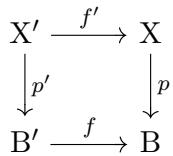
\includegraphics[keepaspectratio]{images/part001_50963eb1.jpg}}

映射 p' 是严格的。

普遍严格映射是严格的。采用定义 6 中的记号，若 \(p\) 是普遍严格的，则 \(p'\) 也是普遍严格的。这由定义立即得出。

推论. --- 开映射、逆紧映射以及具有连续局部截面的映射都是普遍严格的。

例. --- 设 B 为一个拓扑空间，\((\mathrm{A}_{i})_{i\in\mathrm{I}}\) 为 B 的一个覆盖；用 A 表示族 \((\mathrm{A}_{i})_{i\in\mathrm{I}}\) 的和空间，用 \(p: A \to B\) 表示典型映射。在下列两个假设中的每一个之下，映射 p 都是普遍严格的：

\begin{enumerate}
\def\labelenumi{(\roman{enumi})}
\item
  对每个点 \(b \in B\) ，存在 \(i \in I\) ，使得 b 是 \(A_{i}\) 的一个内点；
\item
  族 \((A_{i})\) 是局部有限的，且诸 \(A_{i}\) 是 B 的闭子集。
\end{enumerate}

在假设 (i) 之下，映射 p 在每点的一个邻域内有连续截面。在假设 (ii) 之下，映射 p 按和空间的定义（相应地，由 TG, I, p. 6, prop. 4 与 TG, I, p. 75, th. 1）是逆紧的。因此它是普遍严格的。

注. --- 闭映射未必是普遍严格的 (cf. TG, I, p. 96, exerc. 6)。

命题 11. --- 设

\pandocbounded{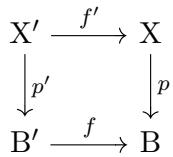
\includegraphics[keepaspectratio]{images/part001_02f1b349.jpg}}

为一个笛卡尔方块。

\begin{enumerate}
\def\labelenumi{\alph{enumi})}
\item
设 f 是严格且满射的。于是，若 p' 是开的（相应地，闭的；相应地，逆紧的），则 p 亦然。
\item
设 f 是闭且满射的。若 p' 是严格的，则 p 是严格的。
\item
设 f 是普遍严格的。若 p' 是普遍严格的，则 p 是普遍严格的。
\end{enumerate}

首先注意，对 X 的每个子集 A，我们有

\[
p ^ {\prime} ((\stackrel {- 1} {f ^ {\prime}}) (\mathrm{A})) = \stackrel {- 1} {f} (p (\mathrm{A})).\tag{20}
\]

事实上，若 \(x' \in (f')^{-1}(\mathrm{A})\) ，则 \(f(p'(x')) = p \circ f'(x') \in p(\mathrm{A})\) 。反之，若 \(b' \in f^{-1}(p(\mathrm{A}))\) ，设 \(x \in A\) 满足 \(f(b') = p(x)\) 。由笛卡尔方块的定义，存在唯一的 \(x' \in X'\) ，使得 \(f'(x') = x\) 且 \(p'(x') = b'\) ，从而 \(b' \in p'((f')^{-1}(\mathrm{A}))\) 。

设 f 是一个开映射且 \(p'\) 是一个严格映射。

集合 \((f')^{-1}(\mathrm{A})\) 在 \(\mathrm{X}'\) 中是开的（相应地，闭的）。于是集合 \(p'((f')^{-1}(\mathrm{A}))\) 在 \(\mathrm{B}'\) 中是开的（相应地，闭的）。由关系式 (20)，它对由 \(f\) 定义的等价关系也是饱和的。由于映射 \(f\) 假设为满射，我们有 \(p(\mathrm{A}) = f(p'((f')^{-1}(\mathrm{A})))\) ，又由于它是严格的，集合 \(p(\mathrm{A})\) 在 B 中是开的（相应地，闭的）。于是映射 \(p\) 是开的（相应地，闭的）。

为使一个连续映射是逆紧的，必须且只需它是闭的且它的纤维是拟紧的 (TG, I, p. 75, th. 1)。若映射 \(p'\) 是逆紧的，则由前所证，映射 \(p\) 是闭的。我们来研究它的纤维：若 \(b \in B\) ，设 \(b' \in B'\) 满足 \(f(b') = b\) 。由 I, p. 10 的推论，映射 \(f'\) 诱导出一个同胚 \(X_{b'}' \to X_b\) 。由于 \(p'\) 是逆紧的，\(X_{b'}'\) 是拟紧的，从而 \(X_b\) 也是。于是映射 \(p\) 是逆紧的。

我们来证明 b) 与 c)。令 \(Y = p(X)\) ，\(Y' = p'(X')\) 。把关系式 (20) 应用于 X，就得到 \(Y' = f^{-1}(Y)\) 。用 g 表示由 f 诱导的从 \(Y'\) 到 Y 中的映射。在情形 b)，由 I, p. 18 的注 1，映射 g 是严格的。在情形 c)，由定义 6 它是严格的，因为方块

\pandocbounded{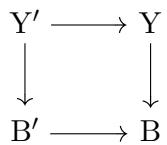
\includegraphics[keepaspectratio]{images/part001_f35053b2.jpg}}

是笛卡尔的。

用 \(q\) 与 \(q'\) 分别表示从 X 到 Y 以及从 \(X'\) 到 \(Y'\) 中的映射，它们由映射 \(p\) 与 \(p'\) 诱导。

\[
\begin{array}{c} \mathrm {X^ {\prime}} \xrightarrow {f ^ {\prime}} \mathrm{X} \\ \Big \downarrow q ^ {\prime} \\ \mathrm {Y^ {\prime}} \xrightarrow {g} \mathrm{Y} \end{array}
\]

由于 \(f\) 是满射，\(f'\) 也是满射；由命题 9 b)，\(p\) 是严格的。

推论 1. --- 设映射 f 是普遍严格且满射的，且映射 p' 是普遍严格的。则映射 p 是普遍严格的。

设

\[
\begin{array}{c} \mathrm{Y} \xrightarrow {g ^ {\prime}} \mathrm{X} \\ \Biggl \downarrow q \\ \mathrm{C} \xrightarrow {g} \mathrm{B} \end{array}
\]

为一个笛卡尔方块；目标是证明映射 q 是严格的。由 I, p. 16 的注 3，方块

\[
\begin{array}{c} \mathrm {X^ {\prime}} \times_ {\mathrm{X}} \mathrm{Y} \xrightarrow {\mathrm{pr} _ {1}} \mathrm {X^ {\prime}} \\ \Biggl \downarrow r \\ \mathrm {B^ {\prime}} \times_ {\mathrm{B}} \mathrm{C} \xrightarrow {\mathrm{pr} _ {1}} \mathrm {B^ {\prime}} \end{array}
\]

和

\[
\begin{array}{c} \mathrm {X^ {\prime} \times_ {X} Y\xrightarrow {pr_ {2}} Y} \\ \Big \downarrow r \\ \mathrm {B^ {\prime} \times_ {B} C\xrightarrow {pr_ {2}} C} \end{array}\tag{21}
\]

都是笛卡尔的，其中 \(r \colon X' \times_{X} Y \to B' \times_{B} C\) 表示由 \((p', q)\) 诱导的映射。由于映射 \(f\) 是普遍严格且满射的，映射 \(\mathrm{pr}_2 \colon B' \times_{B} C \to C\) 亦然 (I, p. 20, def. 6 与 I, p. 10, prop. 4 的推论)。另一方面，映射 \(r\) 是严格的，因为 \(p'\) 假设为普遍严格的。把命题 11 c) 应用于笛卡尔方块 (21)，映射 \(q\) 是严格的。

推论 2. --- 设 B 与 X 为拓扑空间，\(p\colon X \to B\) 为一个连续映射。设 \((A_i)_{i \in I}\) 为 B 的一族子集，它构成 B 的一个开覆盖，或者构成 B 的一个局部有限的闭覆盖。若对每个 \(i \in I\) ，映射 \(p_{A_i}\colon \overline{p}^1(A_i) \to A_i\) 都是严格的（相应地，普遍严格的），则映射 p 是严格的（相应地，普遍严格的）。

对每个 \(i \in \mathrm{I}\) ，令 \(\mathrm{Y}_i = \overline{p}^{1}(\mathrm{A}_i)\) ，\(p_i = p_{\mathrm{A}_i}\) 。设 A 为族 \((\mathrm{A}_i)_{i \in \mathrm{I}}\) 的和空间，Y 为族 \((\mathrm{Y}_i)_{i \in \mathrm{I}}\) 的和空间；用 \(f: \mathrm{A} \to \mathrm{B}\) （相应地，\(g: \mathrm{Y} \to \mathrm{X}\) ，\(q: \mathrm{Y} \to \mathrm{A}\) ）表示由典型单射的族 \(A_i \rightarrow B\) （相应地，典型单射的族 \(Y_i \rightarrow X\) 与诸映射 \(p_i\) ）诱导的映射。方块

\[
\begin{array}{c} \mathrm{Y} \xrightarrow {g} \mathrm{X} \\ \Big \downarrow q \\ \mathrm{A} \xrightarrow {f} \mathrm{B} \end{array}
\]

是一个笛卡尔方块 (例, I, p. 10 与 p. 14)。由 I, p. 20 的推论，映射 \(f\) 是普遍严格的。于是由命题 11，只需证明映射 \(q\) 是严格的（相应地，普遍严格的），如果诸映射 \(p_i\) （\(i \in I\) ）是严格的（相应地，普遍严格的）。这样我们就把该推论的证明化归为这样的情形：诸集合 \(A_i\) （\(i \in I\) ）构成空间 B 的一个由既开又闭的部分组成的分拆，以下即作此假设。

设诸映射 \(p_i\) （\(i \in I\) ）中的每一个都是严格的。若 U 是 X 的一个开子集，且对由 p 定义的等价关系是饱和的，则集合 \(p_i(\mathrm{X}_i \cap \mathrm{U})\) 在 \(\mathrm{A}_i\) 中是开的，从而 \(p(\mathrm{U}) = \bigcup_{i \in \mathrm{I}} p_i(\mathrm{X}_i \cap \mathrm{U})\) 在 B 中是开的。于是映射 p 是严格的。

现在设诸映射 \(p_{i}, i \in I\) 中的每一个都是普遍严格的，我们来证明映射 p 是普遍严格的。设 C 为一个拓扑空间，\(h: C \to B\) 为一个连续映射。目标是证明映射 \(pr_{1}: X \times_{B} C \to C\) 是严格的。空间 C 等同于族 \(C_{i} = h^{-1}(A_{i})\) 的和空间，而空间 \(X \times_{B} C\) 等同于族 \(X \times_{B} C_{i} = X_{i} \times_{A_{i}} C_{i}\) 的直和空间。由于 \(p_{i}\) 是普遍严格的，映射 \(pr_{1}: X_{i} \times_{A_{i}} C_{i} \to C_{i}\) 是严格的。由前所证，映射 \(pr_{1}: X \times_{B} C \to C\) 是严格的。这就证明了映射 p 是普遍严格的。

\section{平展映射}

\subsection{分离映射}

命题 1. --- 设 X 与 Y 为拓扑空间，\(f\colon X \to Y\) 为一个连续映射。下列性质是等价的：

\begin{enumerate}
\def\labelenumi{(\roman{enumi})}
\item
  对角线 \(\Delta_{X}\) （纤维积 X \(\times_{Y}\) X 的）是一个闭子空间；
\item
  对每个拓扑空间 W 与每对从 W 到 X 中的连续映射 \((g_{1}, g_{2})\) （满足 \(f \circ g_{1} = f \circ g_{2}\) ），点 \(w \in W\) （满足 \(g_{1}(w) = g_{2}(w)\) ）所成的集合在 W 中是闭的；
\item
  对每对点 \((x_{1}, x_{2})\) （X 中的），满足 \(x_{1} \neq x_{2}\) 且 \(f(x_{1}) = f(x_{2})\) ，存在一个邻域 \(V_{1}\) （\(x_{1}\) 的，在 X 中）与一个邻域 \(V_{2}\) （\(x_{2}\) 的，在 X 中），使得 \(V_{1} \cap V_{2} = \varnothing\) ；
\end{enumerate}

(i)⇒(ii)：设 \(g_{1}\) 与 \(g_{2}\) 为从 W 到 X 中的连续映射，满足 \(f \circ g_{1} = f \circ g_{2}\) ，并设 \(g: W \to X \times_{Y} X\) 为由 \(g_{1}\) 与 \(g_{2}\) 诱导的映射。由点 \(w \in W\) （满足 \(g_{1}(w) = g_{2}(w)\) ）组成的集合就是 \(g^{-1}(\Delta_{X})\) 。由于 g 是连续的，若对角线 \(\Delta_{X}\) 是闭的，则它是闭的。

(ii)⇒(i)：对角线 \(\Delta_{X}\) 是由点 \(z \in X \times_{Y} X\) （满足 \(\mathrm{pr}_{1}(z) = \mathrm{pr}_{2}(z)\) ）组成的集合。把 (ii) 应用于 \(W = X \times_{Y} X\) 与映射对 \((\mathrm{pr}_{1}, \mathrm{pr}_{2})\) ，即得对角线 \(\Delta_{X}\) 在 \(X \times_{Y} X\) 中是闭的。

(i)⇔(iii)：设 \((x_{1}, x_{2})\) 为 \(X \times_{Y} X\) 的一个点，并设 \(V_{1}\) 与 \(V_{2}\) 分别为 \(x_{1}\) 与 \(x_{2}\) 的邻域。条件 \(V_{1} \cap V_{2} = \varnothing\) 等价于条件 \((\mathrm{V}_{1} \times \mathrm{V}_{2}) \cap \Delta_{\mathrm{X}} = \varnothing\) ，也就是等价于 \((\mathrm{V}_{1} \times \mathrm{V}_{2}) \cap (\mathrm{X} \times_{\mathrm{Y}} \mathrm{X}) \cap \Delta_{\mathrm{X}} = \varnothing\) 。由于诸集合 \((\mathrm{V}_{1} \times \mathrm{V}_{2}) \cap (\mathrm{X} \times_{\mathrm{Y}} \mathrm{X})\) 构成 \((x_{1}, x_{2})\) 在 \(X \times_{Y} X\) 中的一个邻域基，这就证明了 (i) 与 (iii) 的等价性。

定义 1. --- 设 X 与 Y 为拓扑空间。连续映射 \(f: X \to Y\) 称为分离的，如果它满足命题 1 的诸等价条件。

命题 2. --- 设 X、Y、Z 为拓扑空间，\(f\colon X \to Y\) 与 \(g\colon Y \to Z\) 为连续映射。

\begin{enumerate}
\def\labelenumi{\alph{enumi})}
\item
  若 f 与 g 都是分离的，则 \(g \circ f\) 是分离的。
\item
若 g \(\circ\) f 是分离的，则 f 是分离的。
\item
  再设映射 f 是逆紧且满射的。于是，若 g ∘ f 是分离的，则 g 是分离的。
\end{enumerate}

在 X×X 中考虑子空间 \(\Delta_{X}\) （对角线）、\(X \times_Y X\) 与 \(X \times_Z X\) 。它们分别是 X×X 中满足 \(\mathrm{pr}_{1}(u)=\mathrm{pr}_{2}(u)\) 、\(f\circ\mathrm{pr}_{1}(u)=f\circ\mathrm{pr}_{2}(u)\) 、\(g\circ f\circ\mathrm{pr}_{1}(u)=g\circ f\circ\mathrm{pr}_{2}(u)\) 的点 u 所成的集合。若 \(g\circ f\) 是分离的，则 \(\Delta_{X}\) 在 \(X \times_Z X\) 中是闭的，从而在 \(X \times_Y X\) 中也是闭的，由此得 b)。

把命题 1 (ii) 应用于 W = X ×\_Z X、\(g_1 = f \circ \text{pr}_1\) 与 \(g_2 = f \circ \text{pr}_2\) ，则 X ×\_Y X 在 X ×\_Z X 中是闭的，只要 \(g\) 是分离的。此外，若 \(f\) 是分离的，则 \(\Delta_X\) 在 X ×\_Y X 中是闭的 (命题 1, (i))，从而在 X ×\_Z X 中也是闭的，由此得 \(a\) 。

最后，我们来证明 \(c\) 。映射 \((f, f) \colon X \times X \to Y \times Y\) 是逆紧的 (TG, I, p. 73, prop. 4)。子空间 \(X \times_Z X\) 是 \(Y \times_Z Y\) 在 \((f, f)\) 下的原像；由 TG, I, p. 72, prop. 3，映射 \(u \colon X \times_Z X \to Y \times_Z Y\) （由 \((f, f)\) 诱导）是逆紧的。由于 \(g \circ f\) 是分离的，对角线 \(\Delta_X\) 在 \(X \times_Z X\) 中是闭的。于是 \(u(\Delta_X)\) 在 \(Y \times_Z Y\) 中是闭的。由于 \(f\) 是满射，\(u(\Delta_X)\) 是 \(Y \times_Z Y\) 的对角线。这就表明 \(g\) 是分离的。

注. --- 1) 单射的连续映射是分离的。

\begin{enumerate}
\def\labelenumi{\arabic{enumi})}
\setcounter{enumi}{1}
\tightlist
\item
  为使一个拓扑空间 X 是豪斯多夫的 (TG, I, p. 52, def. 1)，必须且只需从 X 到一个化为一点的空间的映射是分离的。在这情形下，从 X 到一个拓扑空间中的每个连续映射都是分离的 (命题 1, (iii))。
\end{enumerate}

设 \(f\colon X \to Y\) 为一个连续且分离的映射。对每个点 \(y\) （\(Y\) 中的），纤维 \(f^{-1}(y)\) 是一个分离的拓扑空间 (loc. cit.)。然而，存在这样的连续映射：它不是分离的，但它的所有纤维都是分离的拓扑空间 (I, p. 140, exerc. 1)。

\begin{enumerate}
\def\labelenumi{\arabic{enumi})}
\setcounter{enumi}{2}
\item
  设 \(f \colon X \to Y\) 为一个连续且分离的映射。若空间 Y 是分离的，则空间 X 是分离的。这由注 2 以及把命题 2 应用于取一个化为一点的空间作为 Z 而得出。
\item
  设 \(f \colon X \to Y\) 为一个连续且分离的映射，\(y\) 为 \(Y\) 的一个点，\(A\) 为 \(f^{-1}(y)\) 的一个有限子集。我们来证明：存在一族两两不相交的集合 \((V_a)_{a \in A}\) ，使得对每个 \(a \in A\) ，集合 \(V_a\) 都是 \(a\) 在 X 中的一个邻域。为此，对每个含两个元素的子集 \(\{a,b\}\) （\(A\) 的），选取一个邻域 \(V_{(a,b)}\) （\(a\) 的）与一个邻域 \(\mathrm{V}_{(b,a)}\) （\(b\) 的，在 X 中），使得 \(\mathrm{V}_{(a,b)} \cap \mathrm{V}_{(b,a)} = \varnothing\) (命题 1, (iii))。用 \(\mathrm{V}_a\) 表示由 X 与诸集合 \(\mathrm{V}_{(a,b)}\) （\(b \in \mathrm{A}\) ，\(b \neq a\) ）组成的族的交。集合 \(\mathrm{V}_a\) 是 \(a\) 在 X 中的一个邻域，且若 \(a\) 、\(b\) 是 A 的两个不同元素，则集合 \(\mathrm{V}_a \cap \mathrm{V}_b\) 包含于 \(\mathrm{V}_{(a,b)} \cap \mathrm{V}_{(b,a)}\) 中，从而是空集。
\item
  设 \(Y\) 为一个拓扑空间。设 \((\mathrm{A}_{i})_{i\in\mathrm{I}}\) 为 Y 的一族子空间，X 为族 \((\mathrm{A}_{i})_{i\in\mathrm{I}}\) 的和空间。从 X 到 Y 的典型映射是分离的。
\end{enumerate}

命题 3. --- 设 \(f\colon X \to Y\) 为一个连续且分离的映射。\(f\) 的每个连续截面都诱导出从 \(Y\) 到 \(X\) 的一个闭子集上的一个同胚。

设 \(s\colon Y \to X\) 为 \(f\) 的一个连续截面。映射 \(s\) 诱导出从 \(Y\) 到子空间 \(s(Y)\) （\(X\) 的）上的一个同胚 (TG, I, p. 22, prop. 9)。\(X\) 的恒等映射与映射 \(s \circ f\) 都是连续的，并且有 \(f \circ \mathrm {Id}_{X} = f \circ (s \circ f)\) 。由于映射 \(f\) 是分离的，集合 \(s(Y)\) ——即由点 \(x\) （在 \(X\) 中且满足 \(x = (s \circ f)(x)\) ）组成的集合——在 \(X\) 中是闭的 (命题 1, (ii))。

命题 4. --- 设

\pandocbounded{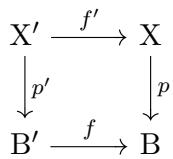
\includegraphics[keepaspectratio]{images/part001_94ec13ba.jpg}}

为一个笛卡尔方块。若映射 p 是分离的，则 p' 亦然。反之，若 p' 是分离的且 f 是普遍严格且满射的，则 p 是分离的。

考虑方块

\[
\begin{array}{c} \mathrm {X^ {\prime} \times_ {B^ {\prime}} X^ {\prime}} \xrightarrow {\varphi} \mathrm {X \times_ {B} X} \\ \Biggl \downarrow_ {q ^ {\prime}} \\ \mathrm {B^ {\prime} \xrightarrow {f} B} \end{array}
\]

其中映射 \(\varphi\) 由映射 \(f' \times f': X' \times X' \to X \times X\) 诱导。回顾 (I, p. 13, 例 1)，这个方块是笛卡尔的，并且有 \(\overline{\varphi}^1(\Delta_X) = \Delta_{X'}\) 。

若映射 p 是分离的，则集合 \(\Delta_{\mathrm{X}}\) 在 \(\mathrm{X} \times_{\mathrm{B}} \mathrm{X}\) 中是闭的；因此 \(\Delta_{\mathrm{X}'}\) 是 \(\mathrm{X}' \times_{\mathrm{B}'} \mathrm{X}'\) 的一个闭子集，这就证明了映射 \(p'\) 是分离的。

若映射 f 是满射的，则映射 \(\varphi\) 是满射的 (I, p. 10, cor.)；若 f 是普遍严格的，则 \(\varphi\) 是严格的 (I, p. 20, def. 6)。设映射 \(p'\) 是分离的。于是 \(\Delta_{\mathrm{X}'}\) 在 \(\mathrm{X}' \times_{\mathrm{B}'} \mathrm{X}'\) 中是闭的。由于 \(\Delta_{\mathrm{X}'} = \overline{\varphi}^{1}(\Delta_{\mathrm{X}})\) 且 \(\varphi\) 是满射且严格的，\(\Delta_{\mathrm{X}}\) 在 \(\mathrm{X} \times_{\mathrm{B}} \mathrm{X}\) 中是闭的，这就证明了映射 \(p\) 是分离的。

命题 5. --- 设 \(f: X \to Y\) 与 \(g: Y \to Z\) 为连续映射。设映射 \(g\) 是分离的且映射 \(g \circ f\) 是逆紧的。则映射 \(f\) 是逆紧的。

考虑下列笛卡尔方块：

\[
\begin{array}{c} \mathrm{X} \times_ {\mathrm{Z}} \mathrm{Y} \xrightarrow {\operatorname{pr} _ {2}} \mathrm{Y} \\ \Biggl \downarrow \operatorname{pr} _ {1} \\ \mathrm{X} \xrightarrow {g \circ f} \mathrm{Z}. \end{array}
\]

设 \(s \colon X \to X \times_{Z} Y\) 为映射 \(x \mapsto (x, f(x))\) 。它是 \(\mathrm{pr}_1 \colon X \times_{Z} Y \to X\) 的一个连续截面。由命题 4，映射 \(\mathrm{pr}_1\) 是分离的；由此推出映射 \(s\) 是逆紧的 (I, p. 27, prop. 3 与 TG, I, p. 72, prop. 2)。另一方面，映射 \(\mathrm{pr}_2\) 是逆紧的 (I, p. 17, prop. 8)。因此，映射 \(f\) （它等于 \(\mathrm{pr}_2 \circ s\) ）是逆紧的 (TG, I, p. 73, prop. 5)。

\subsection{平展映射}

定义 2. --- 设 E 与 B 为拓扑空间，\(p\colon\mathrm{E}\to\mathrm{B}\) 为一个映射，\(x\) 为 E 的一个点。我们称映射 \(p\) 在 \(x\) 处是拓扑平展的，如果存在 \(x\) 在 E 中的一个邻域 U 与 \(p(x)\) 在 B 中的一个邻域 V，使得 \(p\) 诱导出从 U 到 V 上的一个同胚。

我们称映射 p 是拓扑平展的，如果它在 E 的每个点 x 处都是拓扑平展的。

当不致产生混淆时 (cf. 下文例 3)，把拓扑平展简称为平展。代替说 \(p\colon \mathrm{E}\to \mathrm{B}\) 是一个平展映射，也可以说 B-空间 \((\mathrm{E},p)\) 是一个平展 B-空间，或者当映射 \(p\) 无疑问时，简单地说 E 是 B 上的一个平展空间。

注. --- 1) 使映射 \(p \colon \mathrm{E} \to \mathrm{B}\) 平展的 E 的点所成的集合是 E 的一个开子集 U，且 p 在 U 上的限制是一个从 U 到 B 的平展映射。

\begin{enumerate}
\def\labelenumi{\arabic{enumi})}
\setcounter{enumi}{1}
\tightlist
\item
  平展映射是连续且开的 (TG, I, p. 33, prop. 5)；特别地，平展映射的像是开的。反之，若 \(p \colon \mathrm{E} \to \mathrm{B}\) 是一个连续且开的映射，且 E 的每个点 x 都有一个邻域 V 使得映射 \(p \mid \mathrm{V}\) 是单射的，则映射 p 是平展的。平展映射的纤维是离散的。
\end{enumerate}

例. --- 1) 设 B 为一个拓扑空间，\((\mathrm{U}_{i})_{i\in\mathrm{I}}\) 为 B 的一族子集。设 E 表示族 \((\mathrm{U}_{i})_{i\in\mathrm{I}}\) 的和空间，\(p: E \to B\) 表示由诸 \(U_{i}\) 到 B 中的典型单射诱导的映射。为使映射 p 是平展的，必须且只需诸 \(U_{i}\) （\(i \in I\) ）都是开的。

\begin{enumerate}
\def\labelenumi{\arabic{enumi})}
\setcounter{enumi}{1}
\item
为使全纯函数 \(f\colon U \to \mathbf{C}\) 是一个平展映射，必须且只需它的导数不取零值。
\item
  代数簇的平展态射 (VAR, R, 5.7.8) 是一个拓扑平展映射，但存在实代数簇的态射，它是拓扑平展的而不是平展态射。例如，映射 \(x \mapsto x^3\) （从 \(\mathbf{R}\) 到 \(\mathbf{R}\) 中）就是这种情形。然而，一个拓扑平展的复解析簇的态射是平展态射 (I, p. 141, exerc. 6)。
\end{enumerate}

命题 6. — 设 X、Y、Z 为拓扑空间，\(f\colon X\to Y\) 、\(g\colon Y\to Z\) 为映射。

\begin{enumerate}
\def\labelenumi{\alph{enumi})}
\item
  设 f 与 g 都是平展的；则 \(g \circ f\) 是平展的。
\item
  设 \(g\) 是平展的，\(f\) 是连续的且 \(g \circ f\) 是开的。则 \(f\) 是开的。
\item
  设 \(g \circ f\) 与 \(g\) 是平展的，且 \(f\) 是连续的。则映射 \(f\) 是平展的。
\item
  设 \(g \circ f\) 是平展的且映射 \(f\) 是连续且开的；则 \(f\) 是平展的，且 \(g\) 在 \(f(\mathrm{X})\) 的每点处是平展的。
\end{enumerate}

我们来证明 (a)。设 \(f\) 与 \(g\) 都是平展的。于是它们都是连续且开的，从而映射 \(g \circ f\) 是连续且开的。设 \(x\) 为 X 的一个点。存在 \(f(x)\) 在 Y 中的一个邻域 W，使得 \(g \mid \mathrm{W}\) 是单射的，并且存在 \(x\) 在 X 中的一个邻域 V，它包含于 \(f(\mathrm{W})\) 中，使得 \(f \mid \mathrm{V}\) 是单射的；于是映射 \((g \circ f) \mid \mathrm{V}\) 是单射的。这就证明了映射 \(g \circ f\) 是平展的 (注 2)。

我们来证明 b)。设 x 为 X 的一个点，W 为 \(f(x)\) 的一个开邻域，使得 g 诱导出从 W 到开集 \(g(\mathrm{W})\) 上的一个同胚。设 V 为 x 的一个邻域，使得 \(f(\mathrm{V})\) 包含于 W 中；于是 \(g \circ f(\mathrm{V})\) 是 \(g \circ f(x)\) 的一个邻域，因此 \(f(\mathrm{V})\) 是 \(f(x)\) 在开集 W 中的一个邻域，从而也是在 Y 中的一个邻域。这就证明了映射 f 是开的 (TG, I, p. 33, prop. 5)。

我们来证明 c)。由 b)，f 是开的。设 x 为 X 的一个点。由于 \(g \circ f\) 是平展的，存在 x 在 X 中的一个邻域 V，使得 \(g \circ f \mid V\) 是单射的。于是 \(f \mid V\) 是单射的，且 f 是平展的 (I, p. 29, 注 2)。

我们来证明 d)。设 \(x\) 为 \(X\) 的一个点，并令 \(y = f(x)\) 。存在一个开邻域 \(V\) （\(x\) 的），使得 \(g \circ f\) 诱导出从 \(V\) 到开集 \(g \circ f(V)\) 上的一个同胚。由于映射 \(f\) 是开的，\(f(V)\) 是 \(y\) 的一个开邻域。映射 \(f|_V\colon V \to f(V)\) （由 \(f\) 过渡到子空间得到）是连续、开且双射的；因此它是一个同胚，从而 \(f\) 在 \(x\) 处是平展的。此外，映射 \(g\) 诱导出从 \(f(V)\) 到 \(g \circ f(V)\) 上的一个同胚，从而在 \(y\) 处是平展的。

推论 1. — 设 B 为一个拓扑空间。从一个平展 B-空间到另一个平展 B-空间的 B-态射是平展的。

这由命题 6 的断言 c) 得出。

推论 2. --- 设 B 为一个拓扑空间；从一个平展 B-空间到另一个平展 B-空间的双射 B-态射是一个 B-同构。

由推论 1，这样的态射是平展的；因此它是开的 (I, p. 29, 注 2)。若它是双射的，则它是一个 B-同构。

推论 3. --- 设 p: E → B 为一个平展映射。p 的每个连续截面都诱导出从 B 到 E 的一个开子集上的一个同胚。

事实上，这样的截面是平展的 (推论 1)，从而是开的。

推论 4. --- 设 p: E → B 为一个平展且分离的映射。设 E 是连通的且 p 有一个截面。则 p 是一个同胚。

设 \(s\) 为 \(p\) 的一个截面；由于 \(p\) 是平展的，\(s\) 的像在 E 中是开的 (推论 3)；它也是闭的，因为 \(p\) 是分离的 (I, p. 27, prop. 3)。由于 E 是连通的，我们有 \(s(\mathrm{B}) = \mathrm{E}\) ，从而 \(p\) 是一个同胚。

命题 7. --- 设 \(p\colon E \to B\) 为一个连续映射。为使映射 \(p\) 是平展的，必须且只需它是开的，且对角线 \(\Delta_{E}\) （\(E \times_{B} E\) 的）在 \(E \times_{B} E\) 中是开的。

首先设映射 p 是平展的。于是它是开的，且 E 的每个点都有一个邻域 V，使得 \(p|V\) 是单射的，这等于说 \((\mathrm{V} \times \mathrm{V}) \cap (\mathrm{E} \times_{\mathrm{B}} \mathrm{E}) \subset \Delta_{\mathrm{E}}\) 。因此 \(\Delta_{E}\) 是 \(E \times_{B} E\) 的一个开子集。

反之，设 p 是一个开映射且 \(\Delta_{\mathrm{E}}\) 是 \(\mathrm{E} \times_{\mathrm{B}} \mathrm{E}\) 的一个开子集。设 x 为 E 的一个点。设 V 为 x 在 E 中的一个开邻域，使得 \((\mathrm{V} \times \mathrm{V}) \cap (\mathrm{E} \times_{\mathrm{B}} \mathrm{E})\) 包含于 \(\Delta_{\mathrm{E}}\) 中。于是 \(p \mid \mathrm{V}\) 是单射的。由 I, p. 29 的注 2，映射 p 是平展的。

命题 8. --- 设

\pandocbounded{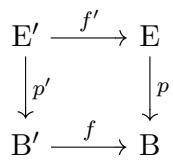
\includegraphics[keepaspectratio]{images/part001_e4ab0ebd.jpg}}

为一个笛卡尔方块。若态射 p 是平展的，则态射 p' 是平展的。反之，若态射 p' 是平展的且态射 f 是普遍严格且满射的，则态射 p 是平展的。

设映射 p 是平展的。特别地，它是开的，且 \(p'\) 是开的 (I, p. 17, prop. 8)。于是考虑笛卡尔方块 (I, p. 13, 例 1)

\[
\begin{array}{c} \mathrm{E} ^ {\prime} \times_ {\mathrm{B} ^ {\prime}} \mathrm{E} ^ {\prime} \xrightarrow {\varphi} \mathrm{E} \times_ {\mathrm{B}} \mathrm{E} \\ \Biggl \downarrow q ^ {\prime} \qquad \qquad \qquad \qquad \Biggl \downarrow q \\ \mathrm{B} ^ {\prime} \xrightarrow {f} \mathrm{B}. \end{array}
\]

我们有 \(\Delta_{\mathrm{E}^{\prime}} = \overline{\varphi}^{1}(\Delta_{\mathrm{E}})\) (loc. cit.)。此外，对角线 \(\Delta_{\mathrm{E}}\) 在 \(\mathrm{E} \times_{\mathrm{B}} \mathrm{E}\) 中是开的 (prop. 7)，从而对角线 \(\Delta_{\mathrm{E}^{\prime}}\) 在 \(\mathrm{E}^{\prime} \times_{\mathrm{B}^{\prime}} \mathrm{E}^{\prime}\) 中是开的。这就证明了映射 \(p^{\prime}\) 是平展的 (loc. cit.)。

现在设映射 \(f\) 是满射且普遍严格的，并设映射 \(p'\) 是平展的。于是 \(p'\) 是开的，因此 \(p\) 是开的 (I, p. 21, prop. 11, \(a\) )。另一方面，\(\Delta_{\mathrm{E}'}\) 是 \(\mathrm{E}' \times_{\mathrm{B}'} \mathrm{E}'\) 的一个开子集。由于 \(\Delta_{\mathrm{E}'} = \overline{\varphi}^{1}(\Delta_{\mathrm{E}})\) 且映射 \(\varphi\) 是满射且严格的 (I, p. 20, def. 6)，\(\Delta_{\mathrm{E}}\) 在 \(\mathrm{E} \times_{\mathrm{B}} \mathrm{E}\) 中是开的。由 prop. 7，映射 p 是平展的。

推论. --- 设 B 为一个拓扑空间。两个平展 B-空间的纤维积是一个平展 B-空间。

设 \((\mathrm{E}, p)\) 与 \((\mathrm{E}^{\prime}, p^{\prime})\) 为平展 B-空间。映射 \(pr_{1}: E \times_{B} E^{\prime} \to E\) 是平展的 (prop. 8)，从而映射 \(p \circ pr_{1}: E \times_{B} E^{\prime} \to B\) 是平展的 (prop. 6, a))。

注 3. --- 设

\pandocbounded{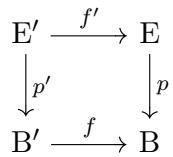
\includegraphics[keepaspectratio]{images/part001_b818a80c.jpg}}

为一个笛卡尔方块。若映射 p 是平展的且映射 f 是严格的，则映射 \(f'\) 是严格的。事实上，在这些假设之下，E 的每个点都有一个开邻域 U，使得 p 诱导出从 U 到开集 \(p(\mathrm{U})\) 上的一个同胚。于是映射 \(p'\) 诱导出从 \((f')^{-1}(\mathrm{U})\) 到 \(f^{-1}(p(\mathrm{U}))\) 上的一个同胚。映射 f 诱导出从 \(f^{-1}(p(\mathrm{U}))\) 到 \(p(\mathrm{U})\) 上的一个严格映射 (I, p. 20)，从而映射 \(f'\) 诱导出从 \((f')^{-1}(\mathrm{U})\) 到 U 中的一个严格映射。由此推出映射 \(f'\) 是严格的 (I, p. 23, 推论 2)。

\subsection{平展映射的局部截面}

设 E 与 B 为集合，A 为 B 的一个子集，\(p: E \rightarrow B\) 为一个映射。p 在 A 上的一个截面是一个映射 \(s: A \rightarrow E\) ，使得 \(p \circ s\) 是 A 到 B 中的典型单射。给出 p 在 A 上的一个截面 s，等价于给出由 p 诱导的映射 \(p_{\mathrm{A}} \colon \overline{p}^{1}(\mathrm{A}) \to \mathrm{A}\) 的一个截面。若 s 是 p 在 A 上的一个截面且 \(A'\) 是 A 的一个子集，则限制 \(s'\) （s 到 \(A'\) 上的）是 p 在 \(A'\) 上的一个截面。这时我们称 s 是 \(s'\) 到 A 上的一个延拓。

当 E 与 B 是拓扑空间且 \(p \colon \mathrm{E} \to \mathrm{B}\) 是连续映射时，集合 \(\mathcal{C}_{\mathrm{B}}(\mathrm{A};\mathrm{E})\) (I, p. 2)（即 \(p\) 在 A 上的连续截面所成的集合）也记作 \(\mathcal{S}(\mathrm{A};p)\) 或 \(\mathcal{S}(\mathrm{A};\mathrm{E})\) 。设 \(s\) 为 \(p\) 在 A 上的一个连续截面。映射 \(s\) 诱导出从 A 到 \(s(\mathrm{A})\) 上的一个同胚，而 \(p\) 诱导出其逆同胚。于是由 I, p. 28 的定义 2，我们有：

命题 9. --- 设 p: E → B 为一个连续映射。为使 p 是平展的，必须且只需 E 的每个点都有一个开邻域，它是在 B 的某个开子集上定义的 p 的一个连续截面的像。

注. --- 1) 设 \(p \colon \mathrm{E} \to \mathrm{B}\) 为一个连续且开的映射。为使 E 的一个开集 U 是 \(p\) 在 B 的某个开集上的一个连续截面的像，必须且只需 \(p\) 在 U 上的限制是单射的。

\begin{enumerate}
\def\labelenumi{\arabic{enumi})}
\setcounter{enumi}{1}
\tightlist
\item
  设 \(p \colon \mathrm{E} \to \mathrm{B}\) 为一个连续映射。设 B 的每个点都有一个开邻域 V，使得存在 \(p\) 在 V 上的一个连续截面。这样的映射 \(p\) 未必是平展的，甚至未必是开的。然而它是满射且普遍严格的 (I, p. 20, 推论)。
\end{enumerate}

\subsection{平展映射的连续提升}

设 \(p \colon \mathrm{E} \to \mathrm{B}\) 与 \(f \colon \mathrm{Z} \to \mathrm{B}\) 为连续映射。\(f\) 到 \(\mathrm{E}\) 中的一个连续提升是指一个连续映射 \(g \colon \mathrm{Z} \to \mathrm{E}\) ，使得 \(p \circ g = f\) 。\(f\) 到 \(\mathrm{E}\) 中的连续提升所成的集合不是别的，正是 \(\mathcal{C}_{\mathrm{B}}(\mathrm{Z};\mathrm{E})\) 。它也可以等同于集合 \(\mathcal{S}(\mathrm{Z};\mathrm{Z} \times_{\mathrm{B}}\mathrm{E})\) ，即 Z-空间 \((\mathrm{Z} \times_{\mathrm{B}}\mathrm{E},\mathrm{pr}_{1})\) 的投影的连续截面所成的集合。

若 T 是 Z 的一个子集，则 f 到 E 中的一个在 T 上定义的连续提升称为 f \textbar{} T 到 E 中的一个连续提升：

\pandocbounded{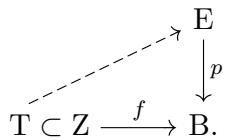
\includegraphics[keepaspectratio]{images/part001_46887bc2.jpg}}

命题 10. --- 设 E、B 与 Z 为拓扑空间，\(p\colon E \to B\) 为一个平展映射，\(f\colon Z \to B\) 为一个连续映射。

设 \(z \in \mathbf{Z}\) 与 \(x \in \mathrm{E}\) 为满足 \(f(z) = p(x)\) 的点。存在一个邻域 \(\mathrm{W}\) （\(z\) 的，在 \(\mathbf{Z}\) 上），以及一个连续提升 \(g\) （\(f\) 的，到 \(\mathrm{E}\) 中），它在 \(\mathrm{W}\) 上定义且满足 \(g(z) = x\) 。

存在 \(p(x)\) 在 B 中的一个开邻域 V 以及 p 在 V 上的一个连续截面 s，使得 \(s(p(x)) = x\) (命题 9)。集合 \(W = f^{-1}(V)\) 是 z 的一个开邻域，而映射 \(g = s \circ (f|W)\) 是 f 到 E 中的一个连续提升，它在 W 上定义且满足 \(g(z) = x\) 。

命题 11. --- 设 E、B 与 Z 为拓扑空间，\(p\colon E \to B\) 与 \(f\colon Z \to B\) 为连续映射。设 \(g\) 与 \(g'\) 为 \(f\) 到 E 中的连续提升。设 W 为 Z 中使 \(g\) 与 \(g'\) 相等的点所成的集合。

\begin{enumerate}
\def\labelenumi{\alph{enumi})}
\item
  若映射 p 是分离的，则 W 是闭的。
\item
  若映射 p 是平展的，则 W 是开的。
\end{enumerate}

用 \(h\) 表示连续映射 \((g, g')\colon Z \to E \times E\) 。\(h\) 的像包含于 \(E \times_{B} E\) 中，因为 \(p \circ g = f = p \circ g'\) ，而 Z 中使 g 与 g' 相等的点所成的集合 W，就是 \(h\) 之下对角线 \(\Delta_{E}\) 的原像。

若映射 p 是平展的，则对角线 \(\Delta_{E}\) 在 \(E \times_{B} E\) 中是开的 (I, p. 31, prop. 7)，从而集合 W 在 Z 中是开的。

若映射 p 是分离的，则对角线 \(\Delta_{E}\) 在 \(E \times_{B} E\) 中是闭的 (I, p. 25, def. 1)，从而集合 W 在 Z 中是闭的。

推论 1. --- 若空间 Z 是连通的且映射 p 是平展且分离的，则在某一点相等的 f 到 E 中的连续提升都相等。

推论 2. --- 设 \(p\colon E \to B\) 为一个分离的平展映射。若空间 E 是连通的，则群 \(\mathrm{Aut}_{\mathrm{B}}(\mathrm{E})\) 自由地作用在 E 上。

事实上，若 \(f: \mathrm{E} \to \mathrm{E}\) 是一个 B-态射，则由推论 1，f 与 \(\mathrm{Id}_{\mathrm{E}}\) 相等的点所成的集合是 E 或空集。

推论 3. --- 设 E、B 与 Z 为拓扑空间，\(p\colon E \to B\) 为一个分离的平展态射，\(f\colon Z \to B\) 为一个连续映射。对 \(i = 1,2\) ，设 \(U_i\) 为 Z 的一个开（相应地，闭）子集，\(g_i\colon U_i \to E\) 为 f 的一个在 \(U_i\) 上定义的连续提升。假设交 \(U_1 \cap U_2\) 是连通的，且存在 \(U_1 \cap U_2\) 的一个点 z，使得 \(g_1(z) = g_2(z)\) 。则存在 f 的一个在 \(U_1 \cup U_2\) 上定义的连续提升，它是 \(g_1\) 与 \(g_2\) 的延拓。

由推论 1，在 \(U_{1} \cap U_{2}\) 上，\(g_{1}\) 与 \(g_{2}\) 的限制相等。映射 \(g: U_{1} \cup U_{2} \to E\) ——由 \(g(z) = g_{i}(z)\) （对 \(z \in U_{i}\) ，i = 1, 2）定义——是 f 的一个在 \(U_{1} \cup U_{2}\) 上定义的连续提升 (TG, I, p. 19, prop. 4)。

在前面的结果中，Z = B 且 \(f = Id_{B}\) 的特殊情形是重要的：这时 f 的连续提升就是 p 的连续截面。

命题 12. --- 设 \(p \colon E \to B\) 为一个平展映射。为使映射 \(p\) 是分离的，必须且只需：对每个开子集 \(V\) （\(B\) 的）与每对 \((s, s')\) （\(p\) 在 \(V\) 上的连续截面的对），使 \(s\) 与 \(s'\) 相等的点所成的集合在 \(V\) 中是闭的。

该条件是必要的 (命题 11, I, p. 34)。我们来证明它是充分的。设 \(b\) 为 B 的一个点，并设 \(x\) 与 \(x'\) 为 E 的两个不同的点，满足 \(p(x) = p(x') = b\) 。设 V 为 b 的一个开邻域，s 与 s' 为 p 在 V 上的连续截面，使得 \(s(\mathrm{V})\) 与 \(s'(\mathrm{V})\) 分别是 x 与 x' 的开邻域 (命题 9)。按假设，由点 \(x \in \mathrm{V}\) （满足 \(s(x) \ne s'(x)\) ）组成的集合 W 在 V 中是开的，从而在 B 中也是开的。集合 \(s(\mathrm{W})\) 与 \(s'(\mathrm{W})\) 分别是 x 与 x' 的开邻域；它们按构造是不相交的。这就证明了映射 p 是分离的 (I, p. 25, 定义 1)。
